\documentclass{article}
\usepackage{amsmath, amssymb, color, xcolor, amsthm}
\usepackage{graphicx, wrapfig, float, caption, dsfont, bbm, xfrac}
\usepackage{fullpage}
\usepackage[backref=page, hidelinks, colorlinks=true, citecolor=blue!60!black!100]{hyperref}
\usepackage{tikz}
\usetikzlibrary{arrows.meta, shapes}
\usepackage{caption, subcaption}
\usepackage{natbib} % gives us \citet: Author (year) and \citep: (Author; year)
\usepackage{authblk}
\usepackage{lineno}
\usepackage{multicol}
\usepackage[bottom]{footmisc}

% for comments in margins or not
\newif\ifmargincomments
\margincommentsfalse
% \margincommentstrue
\ifmargincomments
    \usepackage{todonotes}
    \usepackage[left=1cm,right=6.5cm,top=3cm,bottom=3cm,nohead,nofoot,marginparwidth=6cm]{geometry}
    \newcommand{\plr}[1]{\todo[color=blue!25]{#1}}
    \newcommand{\js}[1]{\todo[color=green!25]{#1}}
    % inline comment version
    \newcommand{\plri}[1]{{\color{blue}\it #1}}
\else
    \newcommand{\plr}[1]{{\color{blue}\it #1}}
    \newcommand{\js}[1]{{\color{green}\it #1}}
    \newcommand{\plri}[1]{\plr{#1}}
\fi

\newcommand{\jss}[1]{{\color{olive}\it #1}}
% \newcommand{\ddt}{\frac{d}{dt}}
\newcommand{\ddt}{\dot}
\newcommand{\ro}{{ro}}
\newcommand{\nro}{{\bar{r}o}}
\newcommand{\rno}{{r\bar{o}}}
\newcommand{\nrno}{{\bar{r}\bar{o}}}
\newcommand{\reachable}{\mathcal{R}}
\newcommand{\unobservable}{\bar{\mathcal{O}}}
\newcommand{\R}{\mathbb{R}}
\newcommand{\E}{\mathbb{E}}
\renewcommand{\P}{\mathbb{P}}
\newcommand{\var}{\mathop{\mbox{Var}}}
\newcommand{\cov}{\mathop{\mbox{Cov}}}
\newcommand{\tr}{\mathop{\mbox{tr}}} % trace
\newcommand{\pda}{\frac{\partial}{\partial A_{ij}}}
\newcommand{\ind}{\mathds{1}}
\newcommand{\grad}{\nabla}

\newcommand{\calH}{\mathcal{H}}
\newcommand{\diag}{\text{diag}}
\newcommand{\1}{\mathbbm{1}}

% the triple (A,B,C) as 'system' (not using)
\newcommand{\Sys}{\mathcal{S}}
% neutral set of all systems
\newcommand{\allS}{\mathcal{N}}

% fitness as a fn of distance
\newcommand{\fit}{\mathcal{F}}
% fitness as a fn of A
\newcommand{\fitx}{\mathcal{F}}
% set of optimal coefficients
\newcommand{\optx}{\mathcal{X}}
% optimal phenotype
\newcommand{\optph}{\Phi_0}
% distance in phenotype space
\newcommand{\dph}{d}
% incompatibility
\newcommand{\Incompat}{\mathcal{I}}

\DeclareMathOperator{\spn}{span}

\newtheorem{theorem}{Theorem}
\newtheorem{lemma}{Lemma}
\newtheorem{definition}{Definition}
\newtheorem{example}{Example}

\begin{document}
%\linenumbers

{\centering
{\LARGE \bf Rapid speciation despite conservation of phenotype} \\ \vspace{0.5cm}
Joshua S. Schiffman$^{\dagger}$ \qquad Peter L. Ralph$^{\dagger \ddagger}$ \\ \vspace{0.5cm}
$^{\dagger}${\footnotesize {Molecular and Computational Biology, University of Southern California, Los Angeles, California 90089, U.S.A. \\
$^{\ddagger}$Departments of Mathematics and Biology \& The Institute for Ecology and Evolution, University of Oregon, Eugene, Oregon 97403, U.S.A.}} \\ \vspace{0.5cm}
{\small \texttt{jsschiff@usc.edu} \qquad 
\texttt{plr@uoregon.edu}} \\ \vspace{0.5cm}
\small \today \\
\vspace{0.25cm}
}

% Other title ideas:
%
% Rapid speciation despite conservation of phenotype
%
% How fast does network drift create incompatibilities?
%
% More than one way to grow a cat: speciation despite conservation of phenotype
%
% More than one way to grow a cat: regulatory network drift and speciation
%
% More than one way to grow a cat: regulatory network redundancy and speciation
%
% Neutral network drift leads to incompatibilities on the same time scale as genetic drift
%
% More than one way to grow a cat: can network drift lead to speciation?
%
% Beyond the snowball: a quantitative model of incompatibility accumulation
%
% System drift and speciation: more than one way to grow a cat
%
% An explicit model of neutral regulatory network evolution, with applications
% to the rate of accumulation of hybrid incompatibility
%
% Evolutionary conservation of phenotype does not entail conservation of the underlying
% molecular mechanism leading to rapid speciation
%
% The evolution of phenotype-invariant gene networks rapidly leads to hybrid incompatibiliy
%
% Evolutionary network rewiring can rapidly lead to hybrid incompatibility despite
% phenotypic conservation
%
% Hybrid incompatibilities can evolve rapidly due to developmental system drift
%
% Evolutionary systems theory and speciation 

\begin{abstract}
%It is known that even if a species' phenotype has remained unchanged over evolutionary time,
%the underlying mechanism may have changed,
%since distinct molecular pathways can realize identical phenotypes.
Even if a species' phenotype remains unchanged over evolutionary time, the underlying mechanism may have changed, as distinct molecular pathways can realize identical phenotypes.
Here we use quantitative genetics and linear system theory to study
how a gene network underlying a conserved phenotype evolves,
as the genetic drift of small mutational changes to these molecular pathways
cause a population to explore the set of mechanisms with identical phenotypes.
% Treating an organism as a ``black box''
To do this, we model an organism's internal state as a linear system of differential equations
for which the environment provides input and the phenotype is the output,
%which translates some environmental input
%to an output that is subject to the pressures of natural selection-- the phenotype.
in which context there exists 
an exact characterization of the set of all mechanisms that give the same input--output relationship.
%There exists an exact expression for the set of all linear mechanisms with identical phenotypes, 
%Due to the genetic drift of small mutational tweaks to these molecular pathways, we expect an evolving population to explore this set.
This characterization implies that selectively neutral directions in genotype space should be common
% there is never a unique network architecture for any phenotype
and that the evolutionary exploration of these distinct but equivalent mechanisms
can lead to the reproductive incompatibility of independently evolving populations.
This evolutionary exploration, or \emph{system drift}, 
proceeds at a rate proportional to the amount of intrapopulation genetic variation
divided by the effective population size ($N_e$).
At biologically reasonable parameter values
this process can lead to substantial interpopulation incompatibility,
and thus speciation, in fewer than $N_e$ generations.
%over a number of generations proportional to the effective population size.
This model also naturally predicts Haldane's rule, 
thus providing another possible explanation
of why heterogametic hybrids tend to be disrupted more often than homogametes during the early stages of speciation.
\end{abstract}

%\plr{Additional ideas to consider adding:}
%\begin{itemize}
%    \item speciation literature
    %\item Haldane's rule (easy point in discussion: makes F1s look like F2s)
    %\item add point about F1: quartic and F2: quadratic to results and maybe abstract/discussion
    %\item hybrid vigor (need to do calculation)
 %   \item discuss linearity, linearization, and canalization in introduction
    %\item obtain estimates of variation in $A$ from thermodynamic occupancy model
 %   \item ``On the origin of species not by means of natural selection''
%\end{itemize}

%\plri{Note: in the \LaTeX source I'm putting in semantic linebreaks, so it's easy to edit and move around phrases and ideas.}

%\plri{Need to come up with a consistent term for ``the $A_{ij}$''s. -- ``regulatory coefficients''? ``genotype''?}

%%%%%%%%%%%%%%%%%%%%%%
%\begin{multicols}{2}
\section*{Introduction}

It is an overarching goal of many biological subdisciplines 
to attain a general understanding of the function and evolution of the 
complex molecular machinery that translates an organism's genome 
into the characteristics on which natural selection acts,
the phenotype.
% Bridging the gulf between an organism's genome and phenotype is a poorly understood and complex molecular machinery. 
%Attaining a general understanding of the functioning and evolution of this molecular machinery
For example, 
there is a growing body of data on the evolutionary histories and molecular characterizations of particular gene regulatory networks
\citep{jaeger2011gap, davidson2006gene, israel2016comparative}, 
as well as thoughtful verbal and conceptual models \citep{true2001developmental, weiss2000phenogenetic, edelman2001degeneracy, pavlicev2012model}. 
Mathematical models of both particular regulatory networks
and the evolution of such systems in general
can provide guidance where intuition fails,
and thus has the potential to discover general principles in the organization of biological systems 
as well as provide concrete numerical predictions \citep{servedio2014not}.

The dynamics of the molecular machinery and its interactions with the environment
can be mathematically described as a dynamical system \citep{jaeger2015comet}.
Movement in this direction is ongoing, as researchers have begun to study 
the evolution of both abstract \citep{wagner1994evolution, wagner1996does, siegal2002waddington, bergman2003evolutionary, draghi2015robustness} 
and empirically inspired computational and mathematical models of gene regulatory networks,
\citep[e.g.][]{mjolsness1991connectionist, jaeger2004dynamic, maria1, vitaly1, vitaly2, crombach2016gap, wotton2015quantitative, chertkova2017insilico}.
% If we allow the reasonable assumption that the genotype-phenotype map 
% can be represented as a system of differential equations \citep{jaeger2015comet}, 
% we can immediately discuss its evolution and function in a much more mechanistic, yet general, manner. 
It is well known that in many contexts mathematical models
can fundamentally be \emph{nonidentifiable} and/or \emph{indistinguishable} -- meaning that 
there can be uncertainty about an inferred model's parameters or even its claims about
causal structure, despite access to complete and perfect data \citep{bellman1970structural, grewal1976identifiability, walter1984structural}. 
Models with different parameter schemes, or even different mechanics 
can make equally accurate predictions,
but still not actually reflect the internal dynamics of the system being modelled.
In control theory, where electrical circuits and mechanical systems are often the focus, 
it is understood that there can be an infinite number of ``realizations'', 
or ways to reverse engineer the dynamics of a ``black box'',
even if all possible input and output experiments on the ``black box'' are performed 
\citep{kalman1963mathematical, anderson1966equivalence, zadeh1976linear}. 
The fundamental nonidentifiability of chemical reaction networks is sometimes referred to as ``the fundamental dogma of chemical kinetics'' \citep{craciun2008identifiability}. 
In computer science, this is framed as the relationship among processes that simulate one another \citep{van2004equivalence}.
Finally,
the field of \emph{inverse problems} studies those cases where,
even if a one-to-one mapping between model and behavior is possible in theory,
even tiny amounts of noise can make inference problems nonidentifiable in practice \citep{petrov2005well}.

Nonidentifiability is a major barrier to mechanistic understanding of real systems, 
but viewed from another angle,
this concept can provide a starting point for thinking about externally equivalent systems
-- systems that evolution can explore, so long as the parameters and structures can be realized biologically.
These functional symmetries manifest in convergent and parallel evolution, 
as well as \emph{developmental system drift}: the observation that
macroscopically identical phenotypes in even very closely related species can in fact be divergent at the molecular and sequence level 
\citep{kimura1981possibility, true2001developmental, tanay2005conservation, tsong2006evolution, hare2008sepsid, lavoie2010evolutionary, vierstra2014mouse, matsui2015regulatory, dalal2016transcriptional, dalal2017transcription}.
Furthermore, theory shows that distinct genotypes encoding identical phenotypes can even persist stably within a species \citep{phillips1996maintenance}.

In this paper we outline a theoretical framework to study the evolution of biological systems, such as gene regulatory networks.
We study the evolution of an optimally adapted population subject to stabilizing selection for phenotype.
Even if the phenotype remains stable over evolutionary time, the underlying mechanism might not remain so,
as many distinct (and mutationally connected) molecular pathways can realize identical phenotypes.
Below, we first apply results from system theory which give
an analytical description of the set of 
all linear gene network architectures that yield identical phenotypes.
Since these phenotypically equivalent gene networks are not necessarily compatible with one another, 
system drift may result in reproductive incompatibility between populations 
isolated for a sufficiently long period of time, 
even in the absence of any sort of adaptive, selective, or environmental change. 
We then use quantitative genetic theory to estimate how quickly 
reproductive incompatibility due to system drift will manifest

 % \jss{should hare2008sepsid be here? It's sequence but not ``system'' drift}
% are these good here? {taylor2016diverse -- maybe not, matsui2015regulatory -- I think this relevant, stergachis2014conservation}.
%
%AND THESE?
  %% Over the last several years, different computational models have been applied to study reproductive incompatibility and speciation in models of gene regulation \citep{porter2002speciation, tulchinsky, palmer2009dynamics, tulchinsky2014hybrid, khatari2015simple}.
  %\citet{tulchinsky} simulated the evolution of a transcription factor and its binding site using a thermodynamic model. Their simulations suggest that the language by which a transcription factor recognizes its binding site can change, and potentially lead to hybrid incompatibility when allopatric populations employ divergent readout languages. This study, despite looking at gene regulation, does not analyze overall gene network architecture -- as we do here -- it only looks at the expression level of a single gene. Furthermore, they report reproductive isolation primarily following directional selection for a change in expression levels in each allopatric population; the evidence for reproductive isolation following balancing selection is much weaker. Johnson and Porter 2000 did not observe any hybrid fitness declines under stabilizing selection -- only under directional selection. 
%Khatari et al, Tulchinsky et al, and Porter et al, all study hybrid incompatibility from a transcription factor/binding site interaction perspective, not from an overall network architecture perspective. Palmer and Feldman only see hybrid incompatibility in constant environments if the parental populations are relatively poorly adapted initially. Otherwise hybrids between two allopatric populations have fairly high fitnesses.  

It is not a new observations that there is often more than one way to do the same thing,
and that this may lead to speciation.
For instance, \citet{tulchinsky2014hybrid}
%(and similarly \citet{khatri2015simple})
looked for hybrid incompatibility
following regulatory sequence drift,
and \citet{porter2002speciation} studied speciation in populations expressing a simple regulatory cascade.
Both found rapid speciation following directional selection,
but only equivocal support for speciation under models of purely neutral drift.
%Additionally, \citet{fierst} observed speciation due to an increase of segregation variance under balancing selection, in models of weak to moderate, but not strong epistasis.
Our model differs from previous work in that we use linear systems theory
to both explore a much richer class of regulatory network models,
and provide analytical expectations in large populations with complex phenotypes
that would be inaccessible to population simulations.
%REFERENCE: Barton's paper (PETER). \citep{barton2010natural}

%%%%%%%%%%%%%%%%%%%%%%%%%%%%%%%%%%%%%
\section*{Results}

We first describe the class of models we study, motivated by gene regulatory networks. 
The behavior (i.e., the temporal dynamics) of such a system is determined by a collection of $n$ coregulating molecules 
-- such as transcription factors -- as well as by external or environmental inputs.
% We model the temporal dynamics of the concentrations of a collection of $n$ coregulating molecules
% within an organism, that may also be affected by temporally varying signals from the environment.
%% Organisms' phenotypes are constructed by gene by gene and gene by environment interactions. 
%%Here we simply define the \emph{phenotype} to be those aspects of the dynamics directly under natural selection
%%-- the \emph{what}, \emph{when}, and \emph{how much}, of an organism's molecules that are physiologically or otherwise relevant to survival.
We write $\kappa(t)$ for the vector of $n$ molecular concentrations at time $t$.
The vector of $m$ ``inputs'' determined exogenously to the system is denoted $u(t)$,
and the vector of $\ell$ ``outputs'' is denoted $\phi(t)$.
The output is merely a linear function of the internal state:
$\phi_i(t) = \sum_j C_{ij} \kappa_j(t)$
for some matrix $C$.
Since $\phi$ is what natural selection acts on, we refer to it as the \emph{phenotype}
(meaning the ``visible'' aspects of the organism),
and in contrast refer to $\kappa$ as the \emph{kryptotype},
as it is ``hidden'' from direct selection.
Although $\phi$ may depend on all entries of $\kappa$,
it is usually of lower dimension than $\kappa$,
and we tend to think of it as the subset of molecules relevant for survival.
The dynamics are determined by
the matrix of regulatory coefficients, $A$,
a time-varying vector of inputs $u(t)$,
and a matrix $B$ that encodes the effect of each entry of $u$ on the elements of the kryptotype.
%Thus an organism's phenotype $\phi(t)$ -- a vector of molecular concentrations at time $t$ -- is determined both by the structure and organization of a biological system (\emph{e.g.} a gene regulatory network), given by the triple $(A,B,C)$,
%and by its environment $u(t)$.
The rate at which the $i^\text{th}$ concentration changes
is a weighted sum of the concentrations of the other concentrations
as well as the input:
\begin{equation}\label{eqn:system}
   \begin{aligned}
    \dot{\kappa}(t) &= A \kappa(t) + B u(t) \\
    \phi(t) &= C \kappa(t) .
  \end{aligned} 
\end{equation}
Furthermore, we always assume that $\kappa(0) = 0$,
so that the kryptotype measures deviations from initial concentrations. 
Here $A$ can be any $n \times n$ matrix, $B$ an $n \times m$, and $C$ any $\ell \times n$ dimensional matrix,
with usually $\ell$ and $m$ less than $n$.
We think of the system as the triple $(A,B,C)$,
which translates (time-varying) $m$-dimensional input $u(t)$ into the $\ell$-dimensional output $\phi(t)$.
Under quite general assumptions,
we can write the phenotype as
  \begin{align}
    \phi(t) = C e^{A t} \kappa(0) + \int_{0}^{t} C e^{A (t-s)} B u(s) ds ,
  \end{align}
which is a convolution of the input $u(t)$ with the system's \emph{impulse response},
which we denote as $h(t) := Ce^{A t}B$.

Although many different biological systems can be modeled with this approach, for clarity, we focus on gene regulatory networks.
In this interpretation, $A_{ij}$ determines how the $j^\text{th}$ transcription factor regulates the $i^\text{th}$ transcription factor.
If $A_{ij} > 0$, then $\kappa_j$ upregulates $\kappa_i$, while if $A_{ij} < 0$, then $\kappa_j$ downregulates $\kappa_i$.
The $i^\text{th}$ row of $A$ is therefore determined by genetic features such as
the strength of $j$-binding sites in the promoter of gene $i$,
factors affecting chromatin accessibility near gene $i$,
or basal transcription machinery activity.
The form of $B$ determines how the environment influences transcription factor expression levels,
and $C$ might determine the rate of production of downstream enzymes.

%% {Linearity} also ``zero-state equivalence''
Here we have assumed that the system is linear,
and begins from the ``zero'' state ($\kappa(0)=0$).
Of course, neither of these are necessarily true for real systems,
but the dynamics of most nonlinear systems can be approximated locally by a linear systems near most points. 
Furthermore, the ease of analyzing linear systems makes this an attractive place to start.
To demonstrate this approach, we apply it to construct a simple gene network in Example \ref{ex:oscillator} below.

\begin{example}[An oscillator]\label{ex:oscillator}
For illustration, we consider an extremely simplified model of oscillating gene transcription,
as for instance is found in cell cycle control or the circadian rhythm.
% Cellular division is governed by many different processes, however it is thought that its rhythm is partially controlled by oscillating gene transcription \citep{orlando2008global}.
There are two genes, 
whose transcript concentrations are given by $\kappa_1(t)$ and $\kappa_2(t)$, 
and gene-2 upregulates gene-1, while gene-1 downregulates gene-2 with equal strength.
Only the dynamics of gene-1 are consequential to the oscillator 
(perhaps the amount of gene-1 activates another downstream gene network). 
Lastly, both genes are equally upregulated by an exogenous signal.
The dynamics of the system are described by
    \begin{align*}
      \dot{\kappa_{1}}(t) &= \kappa_{2}(t) + u(t) \\
        \dot{\kappa_{2}}(t) &= - \kappa_{1}(t) + u(t) \\
        \phi(t) &= \kappa_{1}(t)   .
    \end{align*}
In matrix form the system regulatory coefficients are given as,
$A \!=\! \left[\begin{smallmatrix} 0 & 1 \\ -1 & 0 \end{smallmatrix}\right]$, 
$B \! =\! \left[\begin{smallmatrix} 1 \\ 1 \end{smallmatrix}\right]$,
and $C \!=\! \left[\begin{smallmatrix} 1 & 0 \end{smallmatrix}\right]$.
  %  \begin{align*}
  %    A = \begin{bmatrix} 0 & 1 \\ -1 & 0 \end{bmatrix} , \qquad B = \begin{bmatrix} 1 \\ 1 \end{bmatrix}, \qquad C = \begin{bmatrix} 1 & 0 \end{bmatrix}
  %  \end{align*}
 %       The oscillatory system $\Sigma$ is thus given as
 %   \begin{align*}
 %     \Sigma = \left \{ \begin{array}{ll} \dot{\kappa}(t) &= \begin{bmatrix} 
 %       0 & 1 \\ 
 %      -1 & 0 
 %       \end{bmatrix} \kappa(t) + \begin{bmatrix} 1 \\ 1 \end{bmatrix} u(t) \\ 
 %         \phi(t) &= \begin{bmatrix} 1 & 0 \end{bmatrix} \kappa(t) \end{array} \right.
 %    \end{align*}
Suppose the input is an impulse at time zero (a delta function), and so its phenotype is equal to its impulse response,
\begin{align*}
\phi(t) = h(t) = \sin t + \cos t  .
\end{align*}
The system and its dynamics are referred to in Figure \ref{fig:oscillator}. We return to the evolution of such a system below.   
\end{example}

\begin{figure}[H]
   % \begin{center} 
  \centering
     \begin{tabular}{cc}
        \begin{tikzpicture}
        \begin{scope}[every node/.style={circle,thick,draw}]
            \node (A) at (0,0) {$\kappa_{1}$};
            \node (B) at (4,0) {$\kappa_{2}$};
            \node[shape=rectangle] (U) at (2,2) {input ($u$)};
            \node[shape=rectangle] (y) at (2,-2) {output ($\phi$)};
            %\\  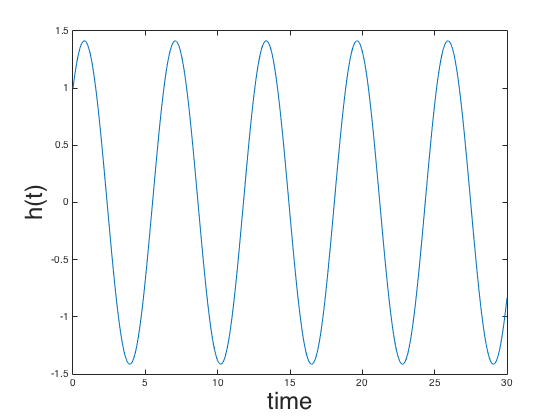
\includegraphics[width=0.15\textwidth, height=0.04\paperheight]{osc_impulse} \end{tabular}};
        \end{scope}

        \begin{scope}[>={Stealth[black]},
                      every node/.style={fill=white,circle},
                      every edge/.style={draw=black, thick}]
            \path [->, >=Rectangle] (A) edge[bend left] node {\tiny $-1$} (B);
            \path [->] (B) edge[bend left] node {\tiny $1$} (A); 
            \path[->] (U) edge node {\tiny $1$} (A);
            \path[->] (U) edge node {\tiny $1$} (B);
            \path[->] (A) edge[bend right] node {\tiny $1$} (y);
        \end{scope}
        \begin{scope}[>={Stealth[black]},
                      every edge/.style={draw=black, thick}]
            %\path [->] (A) edge[loop left] node {\tiny $\lambda_{1}$} (A);
            %\path [->] (B) edge[loop left] node {\tiny $\lambda_{2}$} (B);
        \end{scope}

     \end{tikzpicture} &
   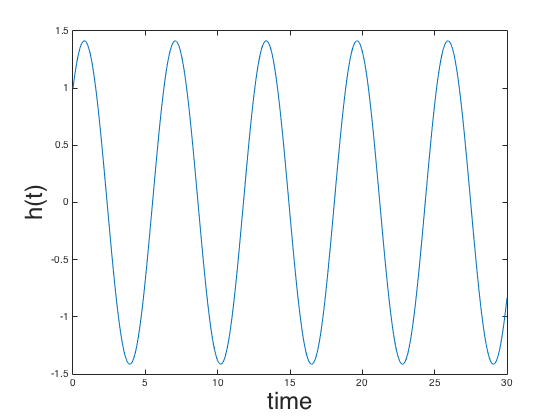
\includegraphics[width=0.5\textwidth, height=0.125\paperheight]{osc_impulse}
\end{tabular}
%  \end{center}
  \caption{
    (Left) 
    Diagram of the gene network in Example \ref{ex:oscillator}
  , and (right) plot of the phenotype $\phi(t)$ against time $t$
  .} \label{fig:oscillator}
\end{figure}


\subsection*{Equivalent gene networks}

As reviewed above,
some systems with identical phenotypes are known to differ, sometimes substantially, at the molecular level; 
systems with identical phenotypes do not necessarily have identical kryptotypes.
How many different mechanisms perform the same function? 

Two systems are equivalent if they produce the same phenotype given the same input,
i.e., have the same input--output relationship.
We say that
the systems defined by $(A,B,C)$ and $(\bar A,\bar B,\bar C)$ are
\textbf{phenotypically equivalent} 
if their impulse response functions are the same:
$h(t) = \bar h(t)$ for all $t \ge 0$.
This implies that for any acceptable input $u(t)$,
if $(\kappa_u(t),\phi_u(t))$ and $(\bar \kappa_u(t),\bar \phi_u(t))$ are the solutions to equation \eqref{eqn:system}
of these two systems, respectively, then
\begin{align*}
      \phi_u(t) = \bar \phi_u(t) \qquad \text{for all} \; t \ge 0.
\end{align*}
% (recall that $\kappa(0) = \bar \kappa(0) = 0$). 
In other words, phenotypically equivalent systems respond identically for \emph{any} input.

One way to find other systems phenotypically equivalent to a given one
is by change of coordinates:
if $V$ is an invertible matrix, then the systems $(A,B,C)$ and $(VAV^{-1},VB,CV^{-1})$
are phenotypically equivalent because their impulse response functions are equal:
  \begin{equation}
    \begin{aligned}
      h(t) &= C e^{A t} B 
      = C V^{-1} V e^{A t} V^{-1} V B \\
      &= C V^{-1} e^{V A V^{-1} t} V B 
      = \bar{C} e^{\bar{A} t} \bar{B} = \bar h(t).
    \end{aligned}
  \end{equation}
However, not all phenotypically equivalent systems are of this form:
systems can have identical impulse responses without being coordinate changes of each other.
In fact, systems with identical impulse responses can involve interactions between different
numbers of molecules, and thus 
have kryptotypes in
different dimensions altogether.

This implies that most systems have at least $n^2$ degrees of freedom,
where recall $n$ is the number of components of the kryptotype vector.
This is because for an arbitrary $n \times n$ matrix $Z$,
taking $V$ to be the identity matrix plus a small perturbation in the direction of $Z$
above implies that
moving $A$ in the direction of $ZA - AZ$
% (e.g., $\bar A = A + \epsilon(ZA-AZ)$)
while also moving $B$ in the direction of $ZB$ 
and $C$ in the direction of $-CZ$
will leave the phenotype unchanged to second order in the size of the perturbation.
%% I believe the following is necessary and sufficient:
If the columns of $B$ and the rows of $C$ are not all eigenvectors of $A$,
then any such $Z$ will result in a different system.

It turns out that in general, there are more degrees of freedom,
except if the system is \emph{minimal} -- meaning, informally, that it uses the smallest possible number of components
to achieve the desired dynamics.
Results in system theory show that any system can be realized in a particular minimal dimension
(the dimension of the kryptotype, $n_\text{min}$),
and that any two phenotypically equivalent systems of dimension $n_\text{min}$ are related by a change of coordinates.
Since gene networks can grow or shrink following gene duplications and deletions, 
these additional degrees of freedom can apply in principle to any system.

Even if the system is not minimal, results from systems theory % -- the Kalman decomposition --
explicitly describe the set of all phenotypically equivalent systems.
% Could define script S here for 'system' if we want: $\Sys$
We refer to $\allS(A_0,B_0,C_0)$ as the set of all systems phenotypically equivalent
to the system defined by $(A_0, B_0, C_0)$:
\begin{equation} \label{eqn:equivalence}
  \begin{aligned}
    \allS(A_0, B_0, C_0) 
      &= \left\{
        (A,B,C) : C e^{At} B = C_0 e^{A_0 t} B_0 \; \text{for}\; t \ge 0 
      \right\}  .
  \end{aligned}
\end{equation}
These systems need not have the same kryptotypic dimension $n$,
but must have the same input and output dimensions ($\ell$ and $m$, respectively).

The Kalman decomposition, which we now describe informally, elegantly characterizes this set
\citep{kalman1963mathematical,kalman1969topics,anderson1966equivalence}.
To motivate this, first note that the input $u(t)$ only directly pushes the system
in certain directions (those lying in the span of the columns of $B$).
As a result, different combinations of input can 
move the system in any direction that lies in what is known as the \emph{reachable subspace}.
Analogously, we can only observe motion of the system in certain directions
(those lying in the span of the rows of $C$),
and so can only infer motion in what is known as the \emph{observable subspace}.
The Kalman decomposition then classifies each direction in kryptotype space
as either reachable or unreachable, and as either observable or unobservable.
Only the components that are both reachable and observable determine the system's phenotype --
that is, components that both respond to an input and produce an observable output. 
% it is possible to add components that respond to an input, 
% but do not influence the output, or components that, in principle, influence the output, but do not respond to any inputs. 

Concretely, the \textbf{Kalman decomposition} of a system $(A,B,C)$  
gives a change of basis $P$ such that
the transformed system $(PAP^{-1},PB,CP^{-1})$  has the following form:
\begin{align*}
       PAP^{-1}
       &=
       \left[ \begin{array}{cccc}
           A_{\rno} & A_{\rno,\ro} & A_{\rno,\nrno} & A_{\rno,\nro} \\
           0 & A_{\ro} & 0 & A_{\ro,\nro} \\
           0 & 0 & A_{\nrno} & A_{\nrno,\nro} \\
          0 & 0 & 0 & A_{\nro}
       \end{array} \right] ,
\end{align*}
and
\begin{align*}
     PB
     &=
    \left[ \begin{array}{cccc}
         B_{\rno} \\
         B_{\ro} \\
         0 \\
         0 
   \end{array} \right] 
   &
   (CP^{-1})^T
   &=
   \left[ \begin{array}{cccc}
       0 \\
       C_{\ro}^T \\
       0 \\
       C_{\nro}^T
   \end{array} \right] .
\end{align*}
% and
% \begin{align*}
%    CP^{-1}
%    &=
%    \left[ \begin{array}{cccc}
%        0 & C_{\ro} & C_{\nrno} & 0 
%    \end{array} \right] .
%\end{align*}
The impulse response of the system is given by
\begin{align*}
      h(t) = C_{\ro} e^{A_{\ro} t} B_{\ro},
\end{align*}
and therefore, the system is phenotypically equivalent to the \emph{minimal} system $(A_{\ro}, B_{\ro}, C_{\ro})$.

This decomposition is unique up to a change of basis that preserves the block structure.
In particular, 
the minimal subsystem obtained by the Kalman decomposition
is unique up to a change of coordinates.
This implies that there is no equivalent system with a smaller number of kryptotypic dimensions
than the dimension of the minimal system.
It is remarkable that the gene regulatory network architecture to achieve a given input--output map is never unique --
both the change of basis used to obtain the decomposition
and, once in this form, all submatrices other than $A_{\ro}$, $B_{\ro}$, and $C_{\ro}$ can be changed without affecting the phenotype,
and so represent degrees of freedom.
(However, some of these subspaces may affect how the system deals with noise.)

\emph{Note on implementation:}
The \emph{reachable subspace},
which we denote by $\reachable$,
is defined to be the closure of $\spn(B)$ under applying $A$,
% (or equivalently, the span of $B, AB, A^2B, \ldots A^{n-1}B$).
% Analogously to this, we define
and the \emph{unobservable subspace}, 
%$\mathcal{O}$, is the closure of $\spn(C^T)$ under applying $A$.
denoted $\unobservable$, is the largest $A$-invariant subspace
contained in the null space of $C$.
% and $\reachable$ is the largest $A$-invariant subspace contained in the image of $B$.)
The four subspaces, $\rno$, $\ro$, $\nrno$, and $\nro$
are defined from these by intersections and orthogonal complements --
$\ro$ refers to the both \emph{reachable and observable} subspace,
while $\nrno$ refers to the \emph{unreachable and unobservable} subspace,
and similarly for $\nro$ and $\rno$.

%Usually, the dimension $n$ and the reference system $\Sys_0$ is implicit and we write only $\calA$.
%Further, we refer to the set of all linear systems with impulse response $h(t)$, regardless of dimension, to be $\allS$,
%  \begin{align}
%    \allS := \bigcup_{n=\min}^{\infty} \calA_n(\Sys_0)
%  \end{align}

For the remainder of the paper, we interpret $\allS$ as the neutral set in the fitness landscape, 
along which a large population will drift under environmental and selective stasis. 
Even if the phenotype is constrained and remains constant through evolutionary time, 
the molecular mechanism underpinning it is not constrained and likely will not be conserved.

Finally, note that if $B$ and $C$ are held constant --
i.e., if the relationships between environment, kryptotype, and phenotype do not change --
there are \emph{still} usually degrees of freedom. 
The following example \ref{ex:all_osc} gives the set of minimal systems equivalent to the oscillator of Example \ref{ex:oscillator},
that all share common $B$ and $C$ matrices.
The oscillator can also be equivalently realized by a three-gene (or larger) network, and will have even more evolutionary degrees of freedom available, 
as in Figure \ref{fig:3D_osc}.

\begin{example}[All phenotypically equivalent oscillators] \label{ex:all_osc}
The oscillator of example \ref{ex:oscillator} is minimal, and so any equivalent system is a change of coordinates
by an invertible matrix $V$.
If we further require $B$ and $C$ to be invariant then we need $VB=B$ and $CV=C$.
Therefore
the following one-parameter family $(A(\tau), B, C)$ describes the set of all two-gene systems
phenotypically equivalent to the oscillator:
    \begin{align*}
      A(\tau) &= \frac{-1}{\tau+1} \begin{bmatrix} -\tau & -1 \\ 2 \tau(\tau + 1) + 1 &  \tau \end{bmatrix} \ \text{for} \ \tau \neq -1 .
    \end{align*}
The resulting set of systems are depicted in Figure \ref{fig:all_osc}.
\end{example}


\begin{figure}[H]
    \centering
\begin{tabular}{cc}
\begin{tikzpicture}
\begin{scope}[every node/.style={circle,thick,draw}]
  \node (A) at (0,0) {$\kappa_{1}$};
    \node (B) at (4,0) {$\kappa_{2}$};
    \node[shape=rectangle] (U) at (2,2) {input ($u$)};
    \node[shape=rectangle] (y) at (2,-2) {output ($\phi$)};
\end{scope}

\begin{scope}[>={Stealth[black]},
              every node/.style={fill=white,circle},
              every edge/.style={draw=black, thick}]
    \path [->, sloped] (A) edge[bend left] node {\tiny $-2 \tau - \frac{1}{\tau+1}$} (B);
    \path [->, sloped] (B) edge[bend left] node {\tiny $\frac{1}{\tau+1}$} (A); 
    \path[->] (U) edge node {\tiny $1$} (A);
    \path[->] (U) edge node {\tiny $1$} (B);
    \path[->] (A) edge[bend right] node {\tiny $1$} (y);
\end{scope}
\begin{scope}[>={Stealth[black]},
              every edge/.style={draw=black, thick}]
    \path [->] (A) edge[loop left] node[left] {\tiny $\frac{\tau}{\tau+1}$} (A);
    \path [->] (B) edge[loop right] node[right] {\tiny $\frac{-\tau}{\tau+1}$} (B);
\end{scope}
\end{tikzpicture} &	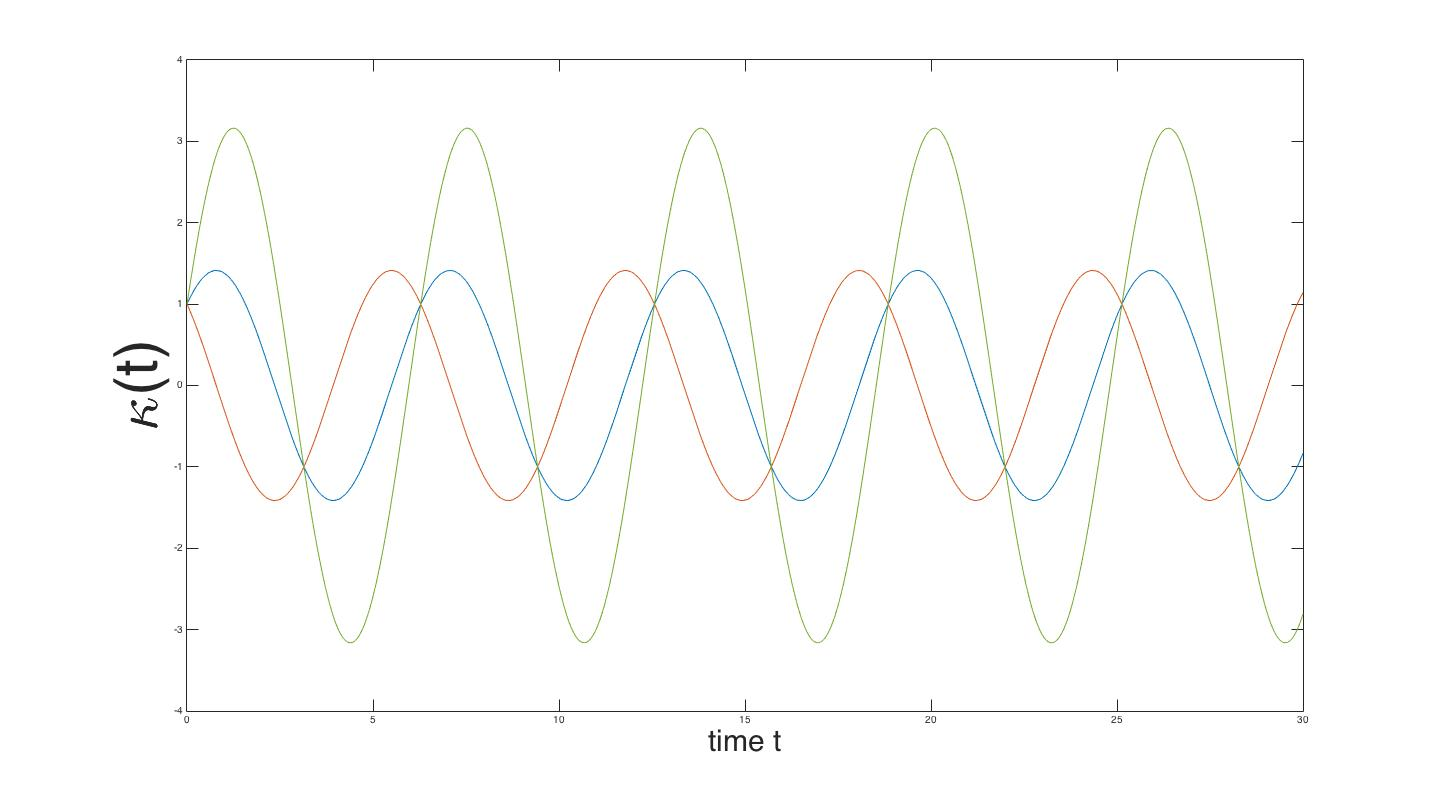
\includegraphics[width=0.5\textwidth, height=0.125\paperheight]{figures/osc_kryp_compare}
    \end{tabular}
% \caption{}
      \caption{
      (Left) $A(\tau)$, the set of all phenotype-equivalent cell cycle control networks.
      (Right) Gene-1 dynamics (blue) for both systems $A(0)$ and $A(-2)$ are identical, however, $A(0)$ gene-2 dynamics (orange) differ from $A(-2)$ (green).
      % Both gene-1 dynamics are given by $\kappa_{1}(t) = \sin t + \cos t$, and gene-2 by $\kappa_{2}(t) = \cos t - \sin t$ ($A(0)$) and $\kappa'_{2}(t) = \cos t + 3 \sin t$ ($A(2)$).
      } 
    \label{fig:all_osc}
\end{figure}


\begin{figure}[H]
    \begin{center}
\begin{tikzpicture}
\begin{scope}[every node/.style={circle,thick,draw}]
  \node (A) at (0,0) {$\kappa_{1}$};
    \node (B) at (0,4) {$\kappa_{2}$};
    \node (C) at (3.464,2) {$\kappa_{3}$};
    \node[shape=rectangle, rotate=0] (U) at (-2.5,2) {input ($u$)};
    \node[shape=rectangle] (y) at (3.464,0) {output ($\phi$)};
\end{scope}

\begin{scope}[>={Stealth[black]},
              every node/.style={fill=white,circle},
              every edge/.style={draw=black, thick}]
    \path [->, sloped] (A) edge[bend left] node {\tiny $2.2$} (B);
   % \path [->, sloped] (B) edge[bend left] node {\tiny ?} (A); 
    \path [->, sloped] (A) edge[bend right] node {\tiny $2$} (C); 
    %\path [->, sloped] (B) edge[bend right] node {\tiny ?} (C); 
    \path [->, >=Rectangle, sloped] (C) edge[bend right] node {\tiny $-1$} (A); 
    \path [->, >=Rectangle, sloped] (C) edge[bend right] node {\tiny $-2.2$} (B); 
    \path[->] (U) edge node {\tiny $1$} (A);
    \path[->] (U) edge node {\tiny $1$} (B);
    \path[->] (A) edge node {\tiny $1$} (y);
\end{scope}
\begin{scope}[>={Stealth[black]},
              every edge/.style={draw=black, thick}]
    \path [->] (A) edge[loop below] node[sloped, below] {\tiny $1$} (A);
    \path [->] (B) edge[loop above] node[sloped, above] {\tiny $1$} (B);
    \path [->, >=Rectangle] (C) edge[loop right] node[sloped, above] {\tiny $-1$} (C);
\end{scope}
\end{tikzpicture}
  \caption{A possible non-minimal three-gene oscillator, phenotypically equivalent to $A(\tau)$, the systems in Examples \ref{ex:oscillator} and \ref{ex:all_osc}.}
  \label{fig:3D_osc}
\end{center}
\end{figure}

\paragraph{Sexual reproduction and recombination}
Parents with phenotypically equivalent yet differently wired gene networks may produce offspring with dramatically different phenotypes. 
If the phenotypes are significantly divergent then the offspring may be inviable or otherwise dysfunctional, 
despite both parents being well adapted. 
If this is consistent for the entire population, we would consider them to be separate species, in accord with the biological species concept \citep{mayr2000biological}.

First, we must specify how sexual reproduction acts on these systems.
Suppose that each of a diploid organisms' two genomes encodes a set of system coefficients.
We assume that a diploid which has inherited systems $(A', B', C')$ and $(A'', B'', C'')$ from its two parents
has phenotype determined by the system that averages these two,
$((A'+A'')/2, (B'+B'')/2, (C'+C'')/2)$.

Each genome an organism inherits is generated by meiosis,
in which both of its diploid parents recombine their two genomes,
and so an $F_1$ offspring carries one system copy from each parent,
and an $F_2$ is an offspring of two independently formed $F_1$s.
If the parents are from distinct populations,
these are simply first-- and second--generation hybrids, respectively.

Exactly how the coefficients 
(i.e., entries of $A$, $B$ or $C$)
of a haploid system inherited by an offspring from her diploid parent
are determined by the parent's two systems
depends on the genetic basis of any variation in the coefficients.
Thanks to the randomness of meiotic segregation,
the result is random to the extent that each parent is heterozygous
for alleles that affect the coefficients.
Since the $i^\text{th}$ row of $A$ summarizes how each gene regulates gene $i$,
and hence is determined by the promoter region of gene $i$,
the elements of a row of $A$ to tend to be inherited together,
which will create covariance between entries of the same row.
It is, however, a quite general observation that the variation seen among recombinant systems
is proportional to the difference between the two parental systems.
This is certainly true if each coefficient is determined by a single nonrecombining locus,
so that each coefficient in the system produced by meiosis is an independent random choice
between the two parental coefficients.
On the other hand, if a coefficient is determined by additive contributions of independently segregating loci,
then the law of total variance applied after conditioning on the parental origin of each allele
implies that the variance is equal to one-quarter of the squared difference between parental coefficients.

Offspring formed from two phenotypically identical systems do not necessarily exhibit the same phenotype as both of its parents -- in other words $\allS$, the set of all systems phenotypically equivalent to a given one, is not, in general, closed under averaging or recombination.
If sexual recombination among systems drawn from $\allS$ yields systems with divergent phenotypes, populations containing significant diversity in $\allS$ can carry genetic load, and isolated populations may fail to produce hybrids with viable phenotypes.


\begin{figure}[H]
\centering
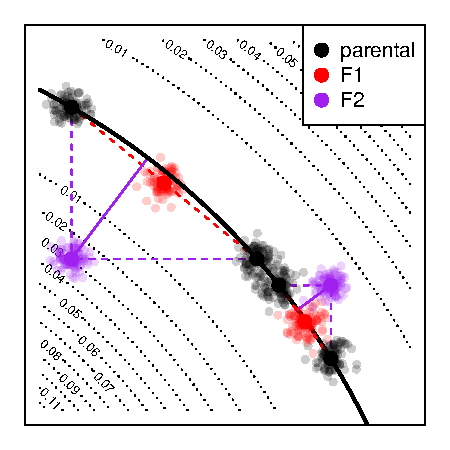
\includegraphics{figures/conceptual_fig}
\caption{
    \label{fig:conceptual_fig}
    A conceptual figure of the fitness consequences of hybridization:
    axes represent system coefficients (i.e., entries of $A$);
    the line of optimal system coefficients is down in black;
    dotted lines give phenotypic distances to the optimum.
    A pair of parental populations are shown in black, along the optimum;
    a hypothetical population of $F_1$s are shown in red,
    and the distribution of one type of $F_2$ is shown in purple
    (other types of $F_2$ are not shown; 
    some would be a similar distance to the other side of the optimal set).
    The distribution of $F_2$ hybrids is appropriate for mixed homozygotes
    if both traits have a simple, one-locus genetic basis,
    but there is variation within each population at that locus.
}
\end{figure}

\subsection*{Hybrid incompatibility}
Two parents with the optimal phenotype can produce offspring whose phenotype is suboptimal
if the parents have different underlying systems.
%This leads to the question: 
How quickly do hybrid phenotypes break down as genetic distance between parents increases?
We will quantify how far a system's phenotype is from optimal
using a weighted difference between impulse response functions.
Suppose that $\rho(t)$ is a nonnegative, smooth, square-integrable weighting function,
$h_0(t)$ is the \emph{optimal} impulse response function
and define the ``distance to optimum'' of another impulse response function
to be
\begin{align}
\label{eqn:distance}
	D(h) = \left( \int_0^\infty \rho(t) \|h(t) - h_0(t)\|^2 dt \right)^{1/2} .
\end{align}
Consider reproduction between a parent with system $(A, B, C)$ 
and another displaced by distance $\epsilon$ in the direction $(X,Y,Z)$,
i.e., having  system $(A + \epsilon X, B + \epsilon Y, C + \epsilon Z)$.
We assume both are ``perfectly adapted'' systems, 
i.e., having impulse response function $h_0(t)$,
and their offspring has impulse response function $h_\epsilon(t)$.
A Taylor expansion of $D(h_\epsilon)$ in $\epsilon$ is explicitly worked out in Appendix \ref{apx:H_calc},
and shows that the phenotype of an $F_1$ hybrid between these two is at distance proportional to $\epsilon^2$ from optimal,
while $F_2$ hybrids are at distance proportional to $\epsilon$.
This is because an $F_1$ hybrid has one copy of each parental system,
and therefore lies directly between the parental systems (see Figure \ref{fig:conceptual_fig}) --
the parents both lie in $\allS$, which is the valley defined by $D$,
and so their midpoint only differs from optimal due to curvature of $\allS$.
In contrast, an $F_2$ hybrid may be homozygous for one parental type in some coefficients
and homozygous for the other parental type in others;
this means that each coefficient of an $F_2$ may be equal to either one of the parents,
or intermediate between the two;
this means that possible $F_2$ systems may be as far from the optimal set, $\allS$,
as the distance between the parents.
The precise rate at which the phenotype of a hybrid diverges depends on the geometry
of the optimal set $\allS$ relative to segregating genetic variation.
% in Figure \ref{fig:conceptual_fig}, this is depicted as the angle of the black line (the optimal set) with respect to the coordinates.

\begin{example}[Hybrid Incompatibility in the Oscillator] \label{ex:hybrid_osc}
Offspring of two equivalent systems from Example \ref{ex:all_osc}
can easily fail to oscillate.
For instance, the $F_1$ offspring between homozygous parents at $\tau=0$ and $\tau=-2$
has phenotype $\phi_{F_1}(t) = e^t$, rather than $\phi(t) = \sin t + \cos t$.
However, the coefficients of these two parental systems differ substantially,
probably more than would be observed between diverging populations.
In figure \ref{fig:hybs} we compare the phenotypes for $F_1$ and $F_2$ hybrids between more similar parents,
and see increasingly divergent phenotypes as the difference between the parental systems increases.
(In this example, the coefficients of $A(\epsilon)$ differ from those of $A(0)$ by an average factor of $1+\epsilon/2$;
such small differences could plausibly be caused by changes to promoter sequences.)
This divergence is quantified in Figure \ref{fig:osc_incompat},
which shows that mean distance to optimum phenotype of the $F_1$ and $F_2$ hybrid offspring between $A(0)$ and $A(\epsilon)$
increases with $\epsilon^2$ and $\epsilon$, respectively.

%% PLR: it says this above already.
% The coefficients in $A$ -- i.e., the regulatory coefficients --
%   differ between parents by only a few percent (around 0.5\% for $\epsilon = - \sfrac{1}{100}$ and 5\% for $\epsilon= - \sfrac{1}{10}$).
% This is well within the amount of regulatory coefficient variation we expect to find segregating within real populations
% (discussed further below). 
% For these small values of $\epsilon$, hybrid phenotypes remain relatively stable, 
%   consistent with the idea that natural selection will allow such intrapopulation variation. For larger values of $\left| \epsilon \right|$ (here $\sfrac{1}{2}$), hybrid phenotypes can become dysfunctional, and depending on context, manifest as hybrid inviability. 

%%% figure of tau=0 and tau=2 hybrid:
%  \begin{figure}[H] 
%    \centering
%    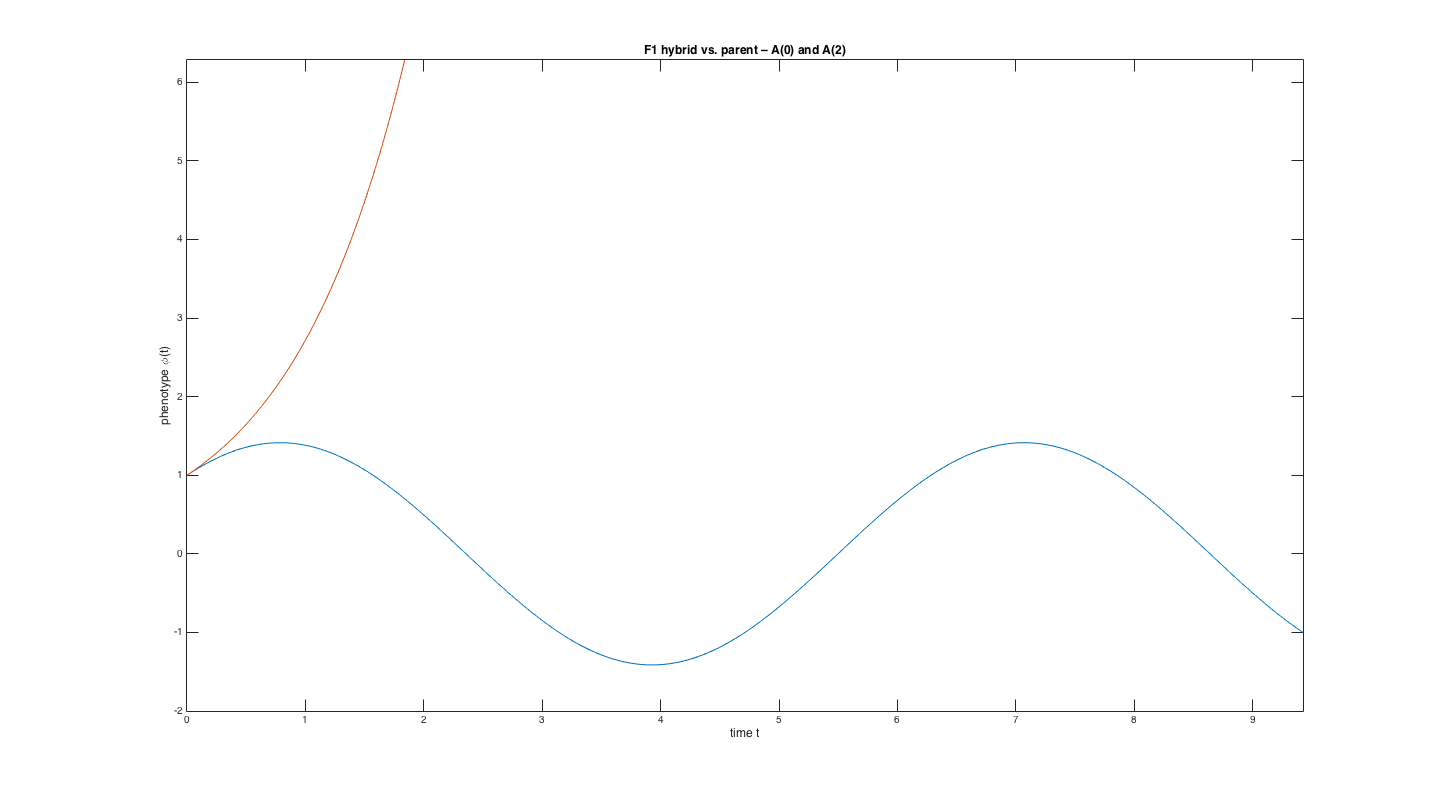
\includegraphics[width=0.5\textwidth, height=0.125\paperheight]{expF1}
%    \caption{\textbf{Hybrid phenotypic breakdown} $F_1$ hybrid (orange) and parental (blue) phenotypic cell-cycle control (oscillator) dynamics %for an $\Sys(0)$ by $\Sys(2)$ cross from Example \ref{ex:all_osc}. The $F_1$ hybrid
%$\left(A_{F_1}\!\!=\!\!\tfrac{A\!(\!0\!) \! + \! A\!(\!2\!)}{2}\right)$
%gene expression fails to oscillate and instead grows exponentialy
%($\phi_{F_0}\! = \! \sin t \! + \! \cos t$, however $\phi_{F_1} \! = \! e^t$).
%    }
%    \label{fig:expF1}
%  \end{figure}


\begin{figure}[H]
  \centering
  \begin{tabular}{ccc}
    %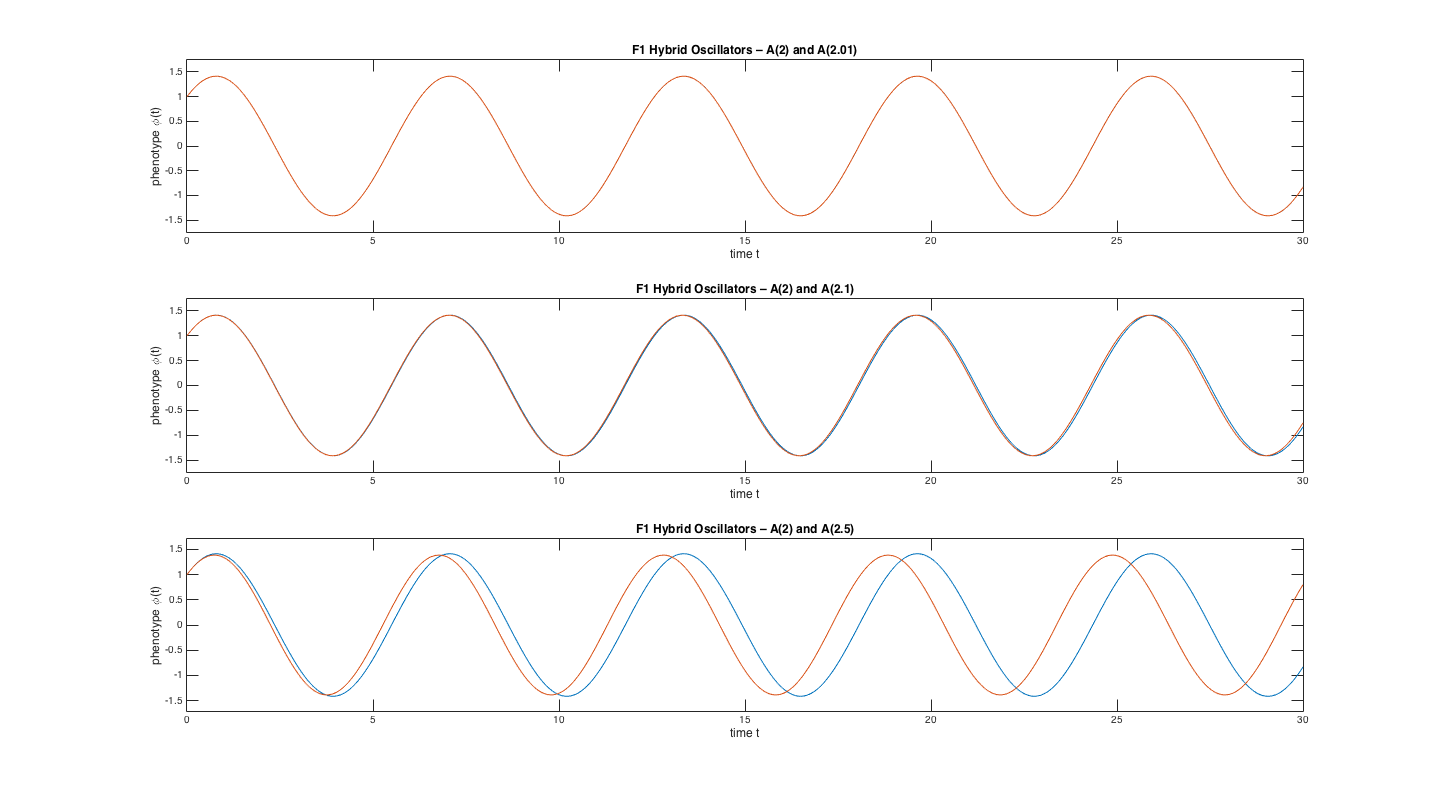
\includegraphics[width=0.5\textwidth, height=0.25\paperheight]{F1_comparison} &
    %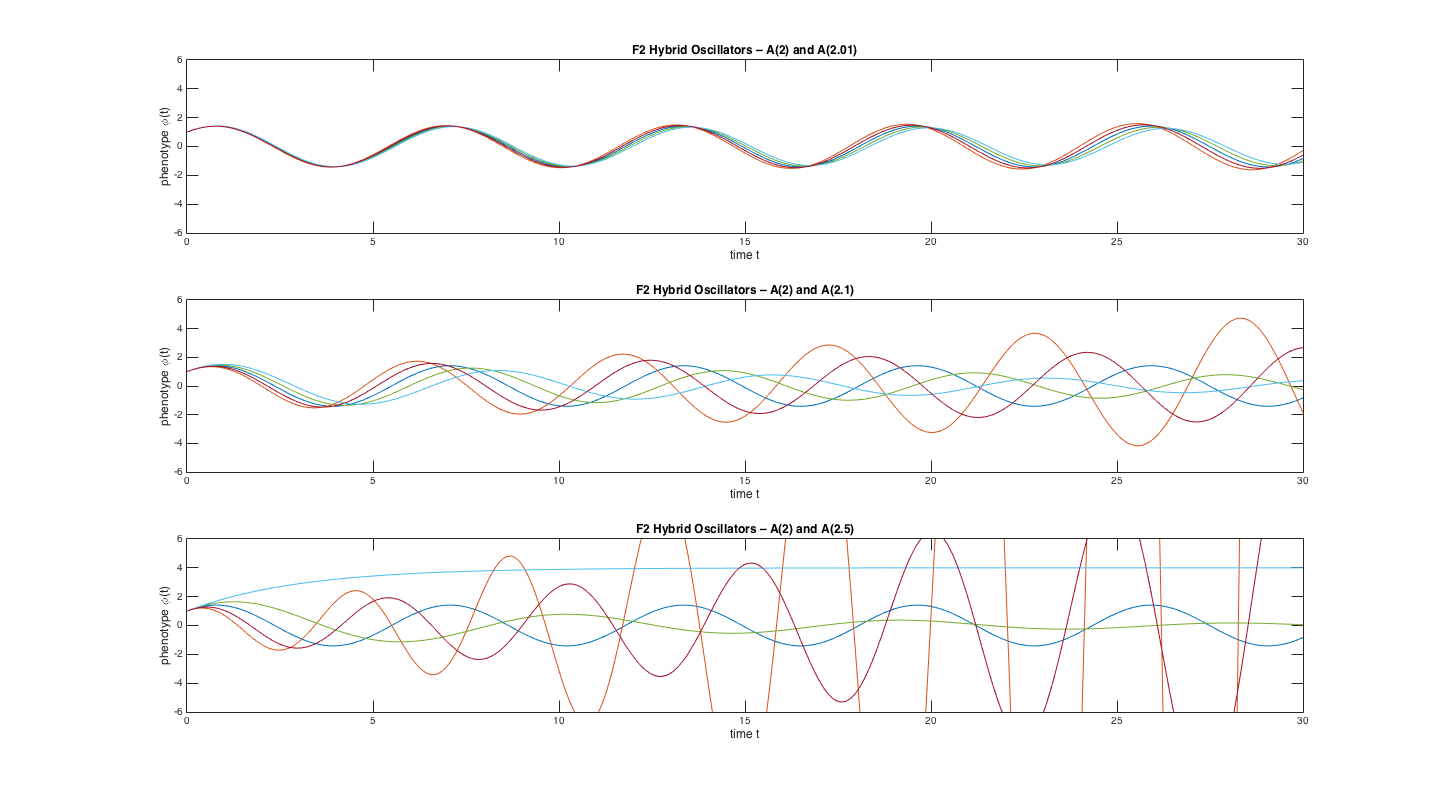
\includegraphics[width=0.5\textwidth, height=0.25\paperheight]{F2s_comparison2}
    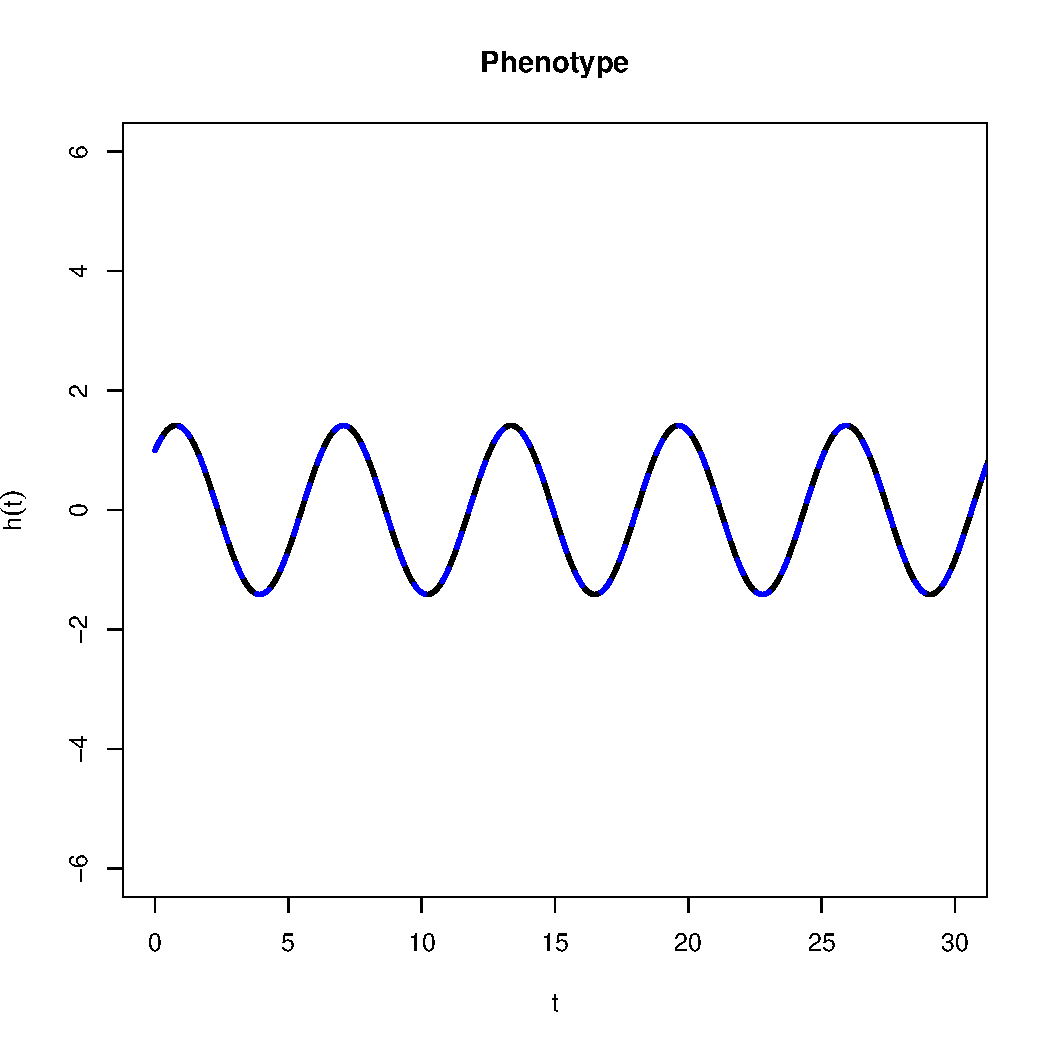
\includegraphics[width=0.5\textwidth, height=0.125\paperheight]{examples/osc_F1_hundreth_tau0} &
      \includegraphics[width=0.5\textwidth, height=0.125\paperheight]{examples/osc_F2_hundrethtau0} \\
      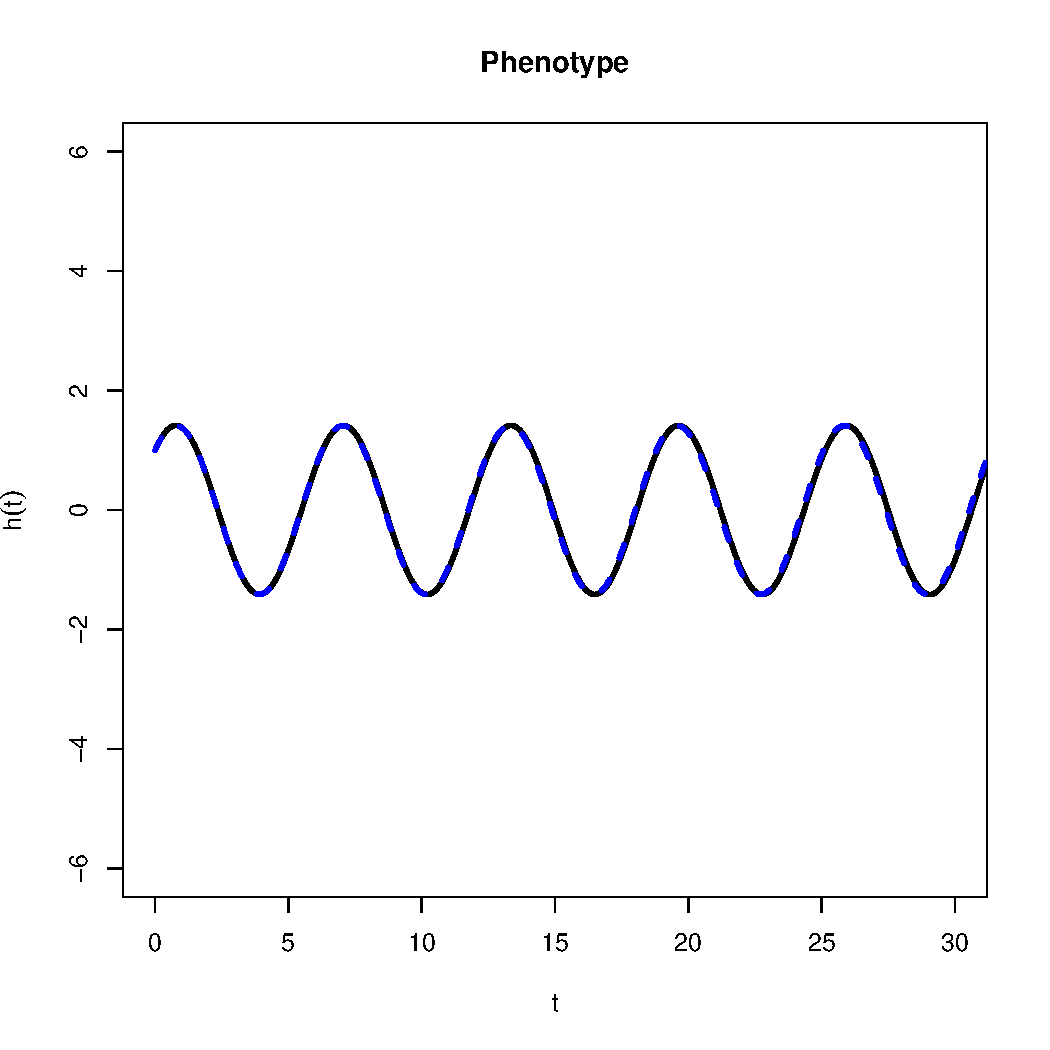
\includegraphics[width=0.5\textwidth, height=0.125\paperheight]{examples/osc_F1_tenth_tau0.pdf} &
      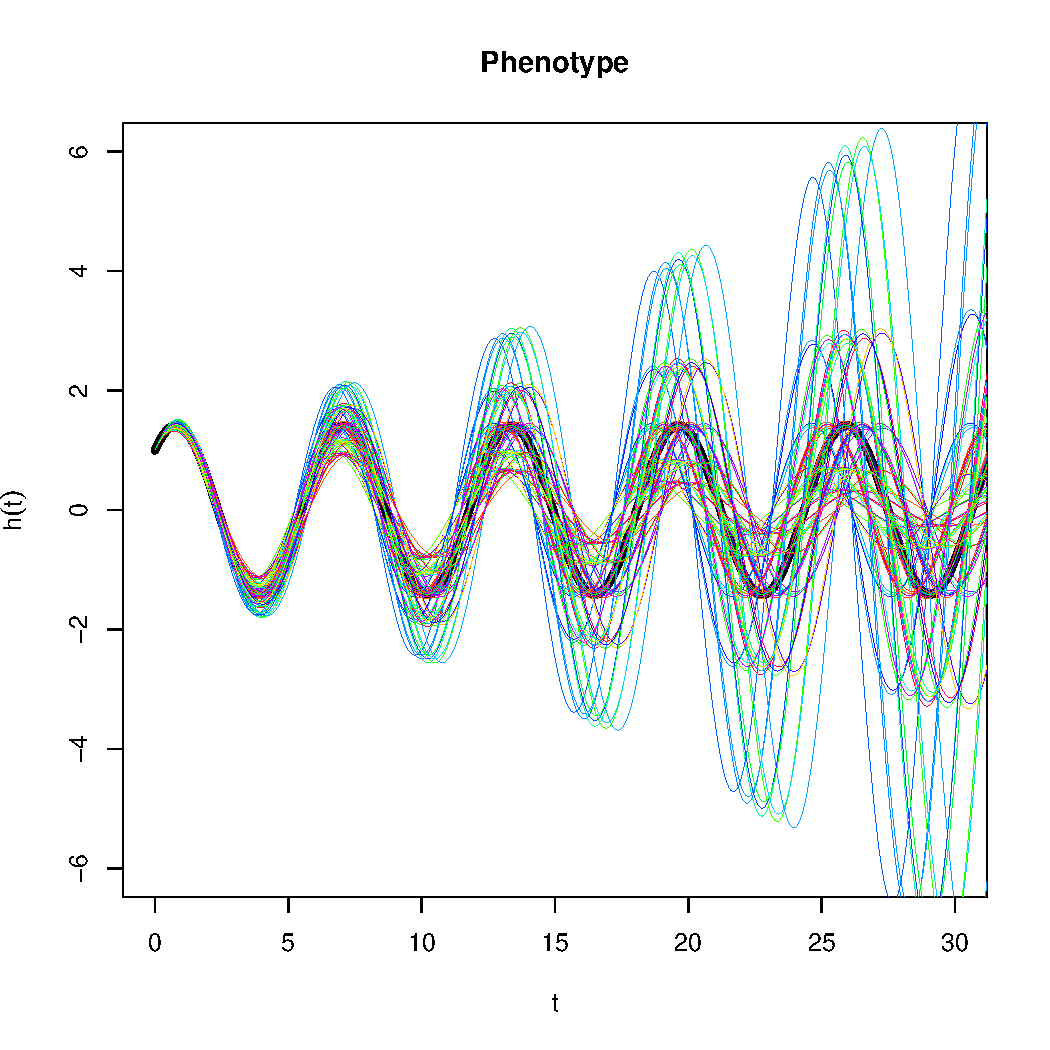
\includegraphics[width=0.5\textwidth, height=0.125\paperheight]{examples/osc_F2_tenthtau0.pdf} \\
      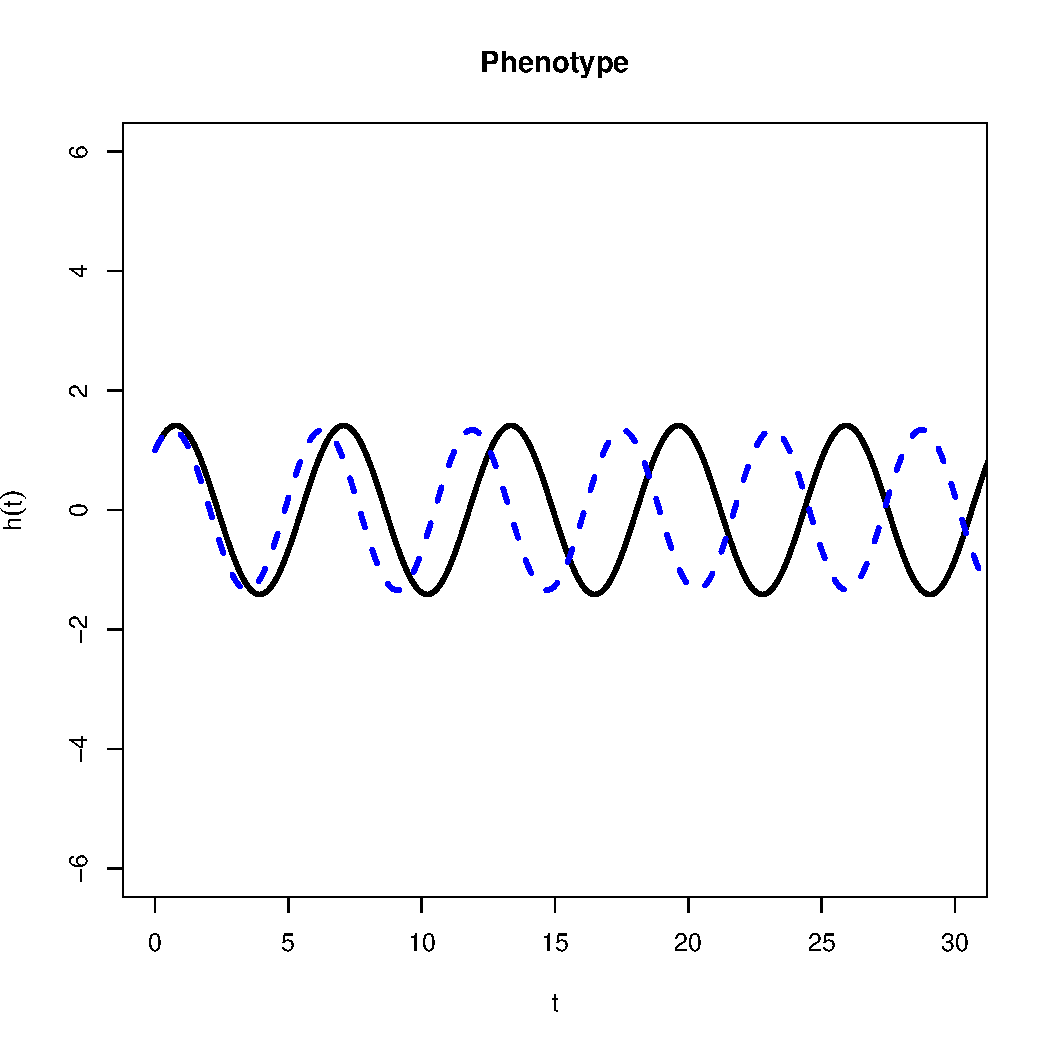
\includegraphics[width=0.5\textwidth, height=0.125\paperheight]{examples/osc_F1_half_tau0.pdf} &
      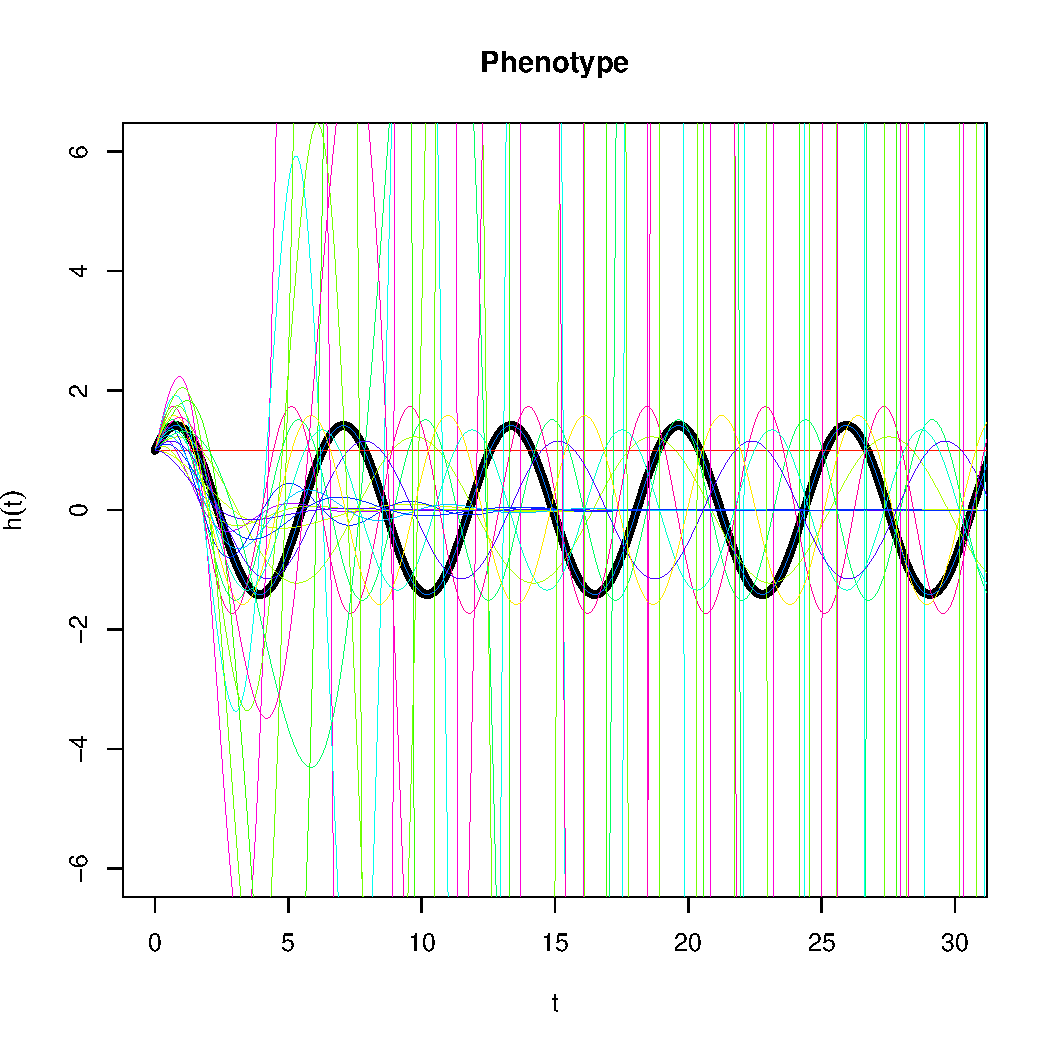
\includegraphics[width=0.5\textwidth, height=0.125\paperheight]{examples/osc_F2_halftau0.pdf}
  \end{tabular}
  \caption{
    \textbf{(left)} Phenotypes of $F_1$ hybrids between an $A(0)$ parent and, top-to-bottom, an $A(\sfrac{1}{100})$, an $A(\sfrac{1}{10})$, and $A(\sfrac{1}{2})$ parent;
    parental coefficients differ by around 0.5\%, 5\%, and 25\% respectively.
    %\plr{These figures are fine; but reparameterize so that the values of $\tau$ are positive.}
    Parental phenotypes ($\sin t + \cos t$) are shown in solid black, and hybrid phenotypes in dashed blue.
    \textbf{(right)} Phenotypes of all possible $F_2$ hybrids between the same set of parents,
    with parental phenotype again in black.
    %% PLR: There are at most 128 possible F2s, not 256; but many are equivalent; 
    %%   it only matters if the offspring is homo/het/homozygous, so there are 3^4 = 81 possible expression patterns.
    Different colored lines correspond to different $F_2$ hybrids;
    note that some completely fail to oscillate.
  } \label{fig:hybs}
\end{figure}

  \begin{figure}[H]
    \centering
    %\begin{tabular}{cc}
    %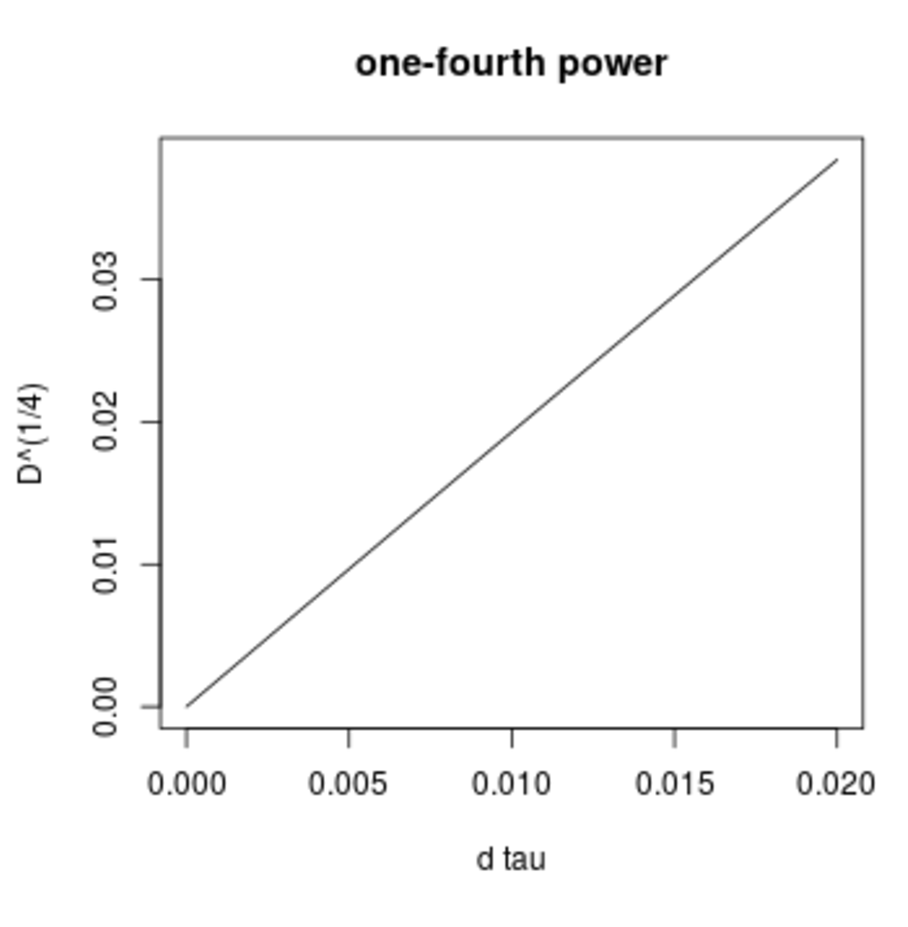
\includegraphics[width=0.4\textwidth]{figures/f1_quartic2} &
    %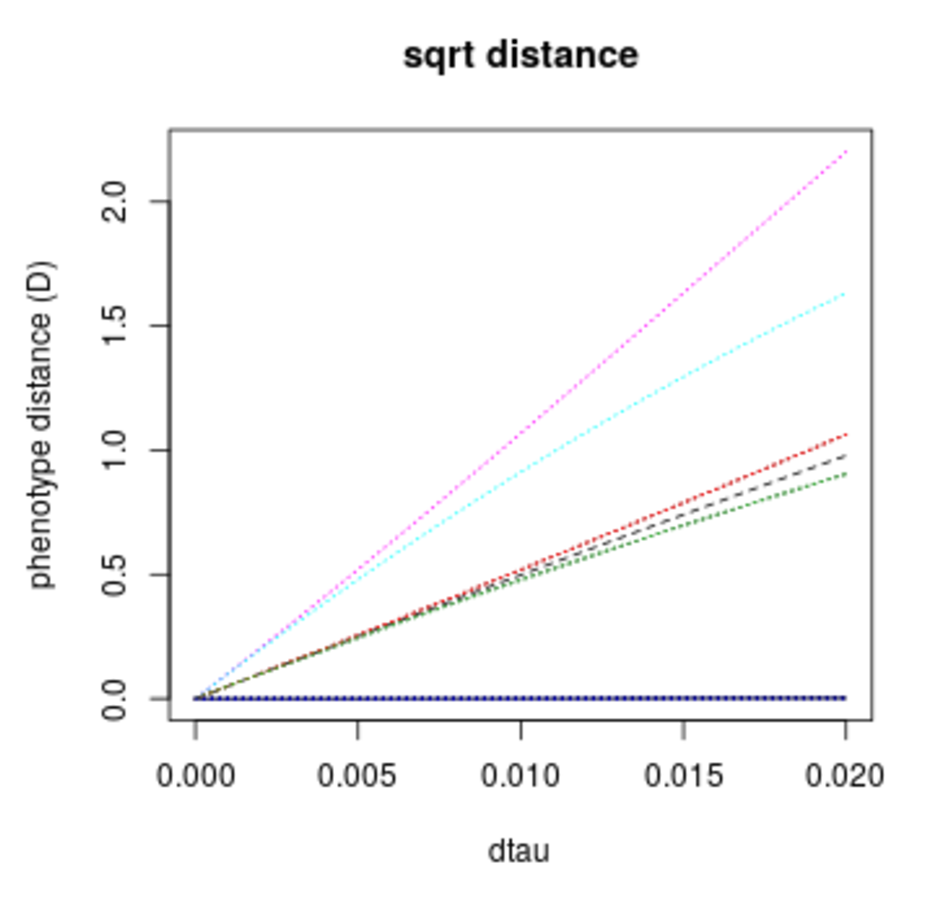
\includegraphics[width=0.4\textwidth]{figures/f2_quad2}
    %\end{tabular}
    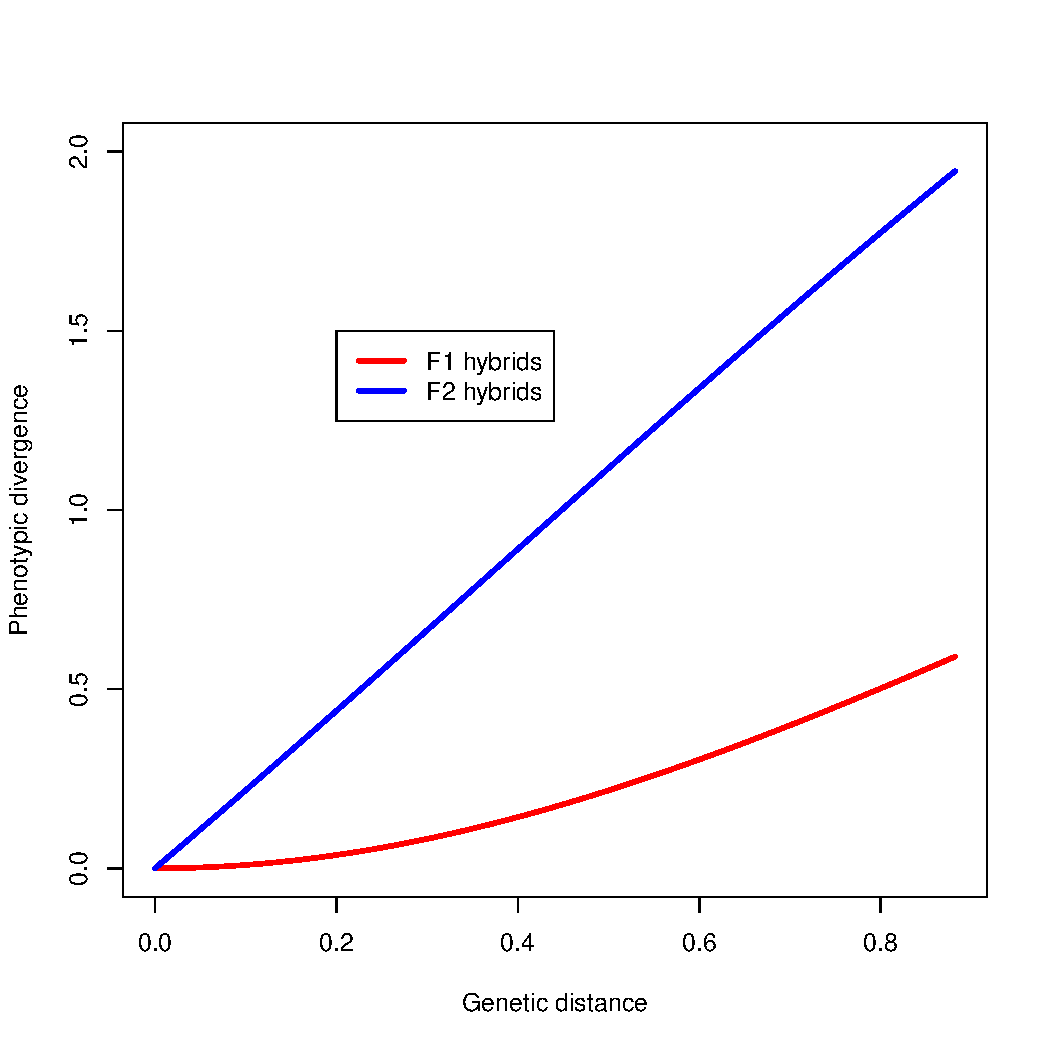
\includegraphics[width=0.5\textwidth]{examples/F2_vs_F1_divergence_tau0}
   % \caption{
    %\textbf{(left)} 
    \caption{Phenotype distance to optimum, $D$, using $\rho(t) = \exp(-t/4\pi)$
    for $F_1$ (black) and $F_2$ (blue) hybrids between an $A(0)$ and an $A(\epsilon)$ parent. Genetic distance is computed as 
    %Frobenius norm
    %Euclidean distance
    $\sqrt{\sum_{ij} (A_{ij}(0) - A_{ij}(\epsilon))^2}$
    %between two systems
    .}
    %\textbf{(right)} Same, but for $F_2$ offspring (one line per type of $F_2$).
    %\plri{make this $D$ not $D^2$ and say which line is the overall average $F_2$.
    %}
    \label{fig:osc_incompat}
  \end{figure}
\end{example}

\paragraph{Haldane's rule}
This model naturally predicts
Haldane's rule, the observation that if only one hybrid sex is sterile or inviable 
it is likely the heterogametic sex (e.g., the male in XY sex determination systems) \citep{haldane1922sex}.
For example, consider an XY species with a two-gene network where the first gene resides on an autosome and the second gene on the X chromosome.
A male whose pair of haplotypes is 
$\left( \left[ \begin{smallmatrix} A_1 & A_2 \\ \cdot & \cdot \end{smallmatrix} \right], \left[ \begin{smallmatrix} A_1 & A_2 \\ X_1 & X_2 \end{smallmatrix} \right] \right)$
has phenotype determined by $A = \left[ \begin{smallmatrix} A_1 & A_2 \\ X_1 & X_2 \end{smallmatrix} \right]$, 
if dosage compensation upregulates heterogametes by a factor of 2 relative to homogametes,
% as in \emph{Drosophila}
while a female homozygous for the haplotype
$\left[\begin{smallmatrix} \bar A_1 & \bar A_2 \\ \bar X_1 & \bar X_2 \end{smallmatrix}\right]$, has phenotype determined by
$A = \left[\begin{smallmatrix} \bar A_1 & \bar A_2 \\ \bar X_1 & \bar X_2 \end{smallmatrix}\right]$.
An $F_1$ male offspring of these two will have its phenotype determined by
$\left[\begin{smallmatrix} (A_1 + \bar A_1)/2 & (A_2 + \bar A_2)/2 \\ \bar X_1 & \bar X_2 \end{smallmatrix}\right]$.
If both genes resided on the autosomes this system would only be possible in an $F_2$ cross.
More generally, 
if the regulatory coefficients for a system are shared between the sex and one or more autosomal chromosomes, 
$F_1$ males are effectively equivalent to purely autosomal-system $F_2$ hybrids. 
In this setting, Haldane's rule is mechanistically similar to \emph{hybrid breakdown}, the observation that $F_2$ hybrids will often be less fit than $F_1$ hybrid crosses, in the early stages of speciation.
This mechanism relies on the genetic variation of a system being shared across the sex chromosomes and the autosomes,
and appears to be distinct from the ``dominance'', ``faster-X'', and ``faster-male'' theories \citep{orr1997haldane, coyne1998evolutionary, turelli1995dominance} usually suggested to explain Haldane's rule.
%and makes several different predictions than the dominance theory as formulated by \citet{turelli1995dominance}.
%\plr{what are they?}
%\citet{turelli1995dominance} employ a population genetic model which strictly requires alleles causing hybrid incompatibility on the X chromosome not to exhibit additive effects, that is the \emph{dominance coefficient} (typically $h$ in classic population genetics) must not be equal to $\frac{1}{2}$. In their model, if alleles are strictly additive, that is neither dominant nor recessive, then male and female $F_1$ hybrids will drop in fitness at the exact same rates, and therefore defy Haldane's rule. 

%%%%%%%%%%%%%%%%%%%%%%%%
\section*{System drift and the accumulation of incompatibilities}

Thus far we have seen that many distinct molecular mechanisms can realize identical phenotypes
and that these mechanisms may fail to produce viable hybrids.
This begs the question: does evolution shift molecular mechanisms
fast enough to be a significant driver of speciation?
To approach this question,
we explore a general quantitative genetic model in which a population drifts stochastically
near a set of equivalent and optimal systems
due to the action of recombination, mutation, and demographic noise.
Although this is motivated by the results on linear systems above,
the quantitative genetics calculations are more general,
and only depend on the presence of genetic variation and a continuous set of phenotypically equivalent systems.

We will suppose that each organism's phenotype is determined by its vector of coefficients, denoted by $x=(x_1, x_2, \ldots, x_p)$,
and that the corresponding fitness is determined by the distance of its phenotype to optimum.
The optimum phenotype is unique, but is realized by many distinct $x$ -- those falling in the ``optimal set'' $\allS$.
The phenotypic distance to optimum of an organism with coefficients $x$ is denoted $D(x)$.
In the results above, $x = (A,B,C)$ and $D(x)$ is given by equation \eqref{eqn:distance}.
The fitness of an organism with coefficients $x$ will be $\exp(-D(x)^2)$.
% this assumption does not entail a loss of generality since $D$ is arbitrary.
We assume that in the region of interest, the map $D$ is smooth
and that we can locally approximate the optimal set $\allS$ as a quadratic surface.
As above, an individual's coefficients are given by averaging its parentally inherited coefficients and adding random noise due to segregation and possibly new mutation.
Concretely, we use the \emph{infinitesimal model} for reproduction \citep{barton2016infinitesimal} --
the offspring of parents at $x$ and $x'$ will have coefficients $(x+x')/2 + \varepsilon$,
where $\varepsilon$ is a random Gaussian displacement due to random assortment of parental alleles.


\paragraph{System drift}
% plr how fast does it drift
We work with a randomly mating population of effective size $N_e$. 
If the population variation has standard deviation $\sigma$ in a particular direction,
since subsequent generations resample from this diversity,
the population mean coefficient will move a random distance of size $\sigma/\sqrt{N_e}$ per generation,
simply because this is the standard deviation of the mean of a random sample \citep{lande1981models}.
% (This could be taken as a definition of $N_e$.)
Selection will tend to restrain this motion,
but movement along the optimal set $\allS$ is unconstrained,
and so we expect the population mean to drift along the optimal set like a particle diffusing.
% (although perhaps complicated by recombination load \citep{recomb_load})
The amount of variance in particular directions in coefficient space 
depends on constraints imposed by selection and 
correlations between the genetic variation underlying different coefficients 
(the $G$ matrix \citep{arnold2008understanding}).
It therefore seems reasonable to coarsely model the time evolution of population variation in regulatory coefficients as 
a ``cloud'' of width $\sigma$ about the population mean, 
which moves as an unbiased Brownian motion through the set of network coefficients that give the optimal phenotype.

% covariance which may arise due to functional constraints and/or statistical linkage.
% There may well be functional constraints -- but these are not sufficiently well-known to say anything general about.
%For instance,
%if the variation is due to \textit{cis}-regulatory variants,
%the genetic basis of each \emph{row} of $A$ likely lies within a few kilobases of tightly linked sequence,
%across which a population may carry only a few common haplotypes.
%However, covariance due to transiently assembled haplotypes is not expected to be stable over long periods of time --
%a common \textit{cis}-regulatory haplotype of transcription factor $k$ with particularly strong binding to both $i$ and $j$
%(leading to positive covariance between $A_{ik}$ and $A_{jk}$)
%is no more likely to appear than one with strong binding to $i$ but particularly weak binding to $j$ (negative covariance).
%(Such transient covariances may well increase the variance of the per-generation change in network mean, however \citep{barton_linkage}.)

Next, we calculate with some simplifying assumptions to give the general idea;
multivariate derivations appear in Appendix \ref{ss:quant_gen}.
There will in general be different amounts of variation in different directions;
to keep the discussion intuitive, we only discuss $\sigma_N$, the amount of variation in ``neutral'' directions
(i.e., directions along $\allS$),
and $\sigma_S$, the amount of variation in ``selected'' directions (perpendicular to $\allS$).
The other relevant scale we denote by $\gamma$,
which the scale on which distance to phenotypic optimum changes as $x$ moves away from the optimal set, $\allS$.
Concretely, $\gamma$ is
%the inverse of the derivative of 
$1/(\frac{d}{du}D(x+uz))$ 
where $x$ is optimal and $z$ is a ``selected'' direction perpendicular to $\allS$.
With these parameters, a typical individual will have a fitness of around $\exp(-(\sigma_S/\gamma)^2)$.
Of course, there are in general many possible neutral and selected directions;
we take $\gamma$ to be an appropriate average over possible directions.

\paragraph{Hybridization}
The means of two allopatric populations each of effective size $N_e$ separated for $T$ generations
will be a distance roughly of order $2\sigma_N \sqrt{T/N_e}$ apart along $\optx$.
(Consult figure \ref{fig:conceptual_fig} for a conceptual diagram.)
A population of $F_1$ hybrids has one haploid genome from each,
whose coefficients are averaged,
and so will have mean system coefficients at the midpoint between their means.
The distribution of $F_2$ hybrids will have mean at the average of the two populations,
but will have higher variance.
The variance of $F_2$ hybrids can be shown to increase linearly with the square of the distance between
parental population means
under models of both simple and polygenic traits.
This is suggested by figure \ref{fig:conceptual_fig} and shown in Appendix \ref{apx:seg_cov}.
Concretely, we expect the population of $F_1$s to have variance $\sigma^2_S$ in the selected direction
(the same as within each parental population),
but the population of $F_2$ hybrids will have variance of order $\sigma^2_S + 4 \omega \sigma^2_N T/N_e$,
where $\omega$ is a factor that depends on the genetic basis of the coefficients.
If the optimal set $\allS$ has dimension $q$,
using the polygenic model of appendix \ref{apx:seg_cov}, 
$\omega$ is proportional to the number of degrees of freedom: $\omega = (p-q)/8$.
If each trait is controlled by a single locus, as in figure \ref{fig:conceptual_fig},
the value is similar.

%%% CITE SOME OF THESE
%% empirical data on sigma
% The amount and structure of this standing variation is established over long time scales
% by many factors, including mutation-selection balance, 
% shifts in the phenotypic optimum, and/or spatial variation in the optimum \citep{hansen1996translating}.
% Quantitative genetics models of mutation-selection balance 
% predict precise levels and structure of standing variation \citep{kimura_mutsel,lande_mutsel,lande1981models},
% but it is unclear how well these predictions match reality \citep{johnson_barton}
% and how much they are expected to change over time \citep{arnold_changing_G}.

What are the fitness consequences?
A population of $F_2$ hybrids will begin to be substantially less fit than the parentals
once they differ from the optimum by a distance of order $\gamma$,
i.e., once $\sqrt{4 \omega T/N_e} \approx \gamma / \sigma_N$.
This implies that hybrid incompatibility among $F_2$ hybrids should appear much slower --
on a time scale of $N_e (\gamma / \sigma_N)^2 / (4 \omega)$ generations.
The $F_1$s will not suffer fitness consequences until the hybrid mean is further than $\gamma$ from the optimum;
as shown in appendix \ref{apx:away_from_opt} (and suggested by figure \ref{fig:conceptual_fig}),
this deviation of the mean from optimum grows with the square of the distance between the parental populations,
and so we expect fitness costs in $F_1$s to appear on a time scale of $N_e^2$ generations.

% If a population has a Gaussian distribution of trait values with variance $\sigma^2$
% and fitness decays as $\exp(-x^2/2\gamma)$ away from the population mean,
% then the population mean fitness is 
% \begin{align*}
%    \int \frac{1}{\sigma \sqrt{2\pi}} e^{-\frac{x^2}{2\sigma^2}} e^{-\frac{x^2}{2\gamma^2}} dx
%    &=
%    \sqrt{\frac{1}{1 + (\sigma/\gamma)^2}}  \le \frac{1}{\sigma/\gamma} .
% \end{align*}
% If $\sigma$ is much smaller than $\gamma$, the fitness consequences of variation
% (i.e., genetic load) are small,
% but if $\sigma$ is of order $\gamma$, then mean fitness is inversely proportional to trait variance
% (i.e., $\gamma/\sigma$).
% This implies that we expect $\sigma_S < \gamma$
% but that once $T$ is of order $N_e (\gamma / \sigma_H)^2$, there will be loss of fitness
% in $F_2$ hybrids.
% Said another way,
% if we write $\mathcal{F}(T)$ as the mean fitness of an $F_2$ hybrid between two populations separated by $T$ generations,
% then fitness drops with the square root of $T$, measured in units of $N_e$ generations:
% \begin{align*}
%    \mathcal{F}(T) \le \frac{1}{\sigma_H/\gamma}\sqrt{\frac{N_e}{T}} .
% \end{align*}

For a more concrete prediction, suppose that the distribution among hybrids is Gaussian.
A population whose trait distribution is Gaussian with mean $\mu$ and variance $\sigma$,
has mean fitness 
\begin{align} \label{eqn:gauss_fit}
\int_{-\infty}^\infty \frac{1}{\sigma\sqrt{2\pi}} e^{-\frac{(x-\mu)^2}{2\sigma^2}} e^{-\frac{x^2}{2\gamma^2}} dx
&=
\sqrt{\frac{1}{1 + \sigma^2/\gamma^2}} \exp\left\{-\frac{\mu^2}{\gamma^2}\left(\frac{1}{1 + \sigma^2/\gamma^2}\right)\right\} .
% &\approx
% \frac{1}{\sigma/\gamma}\left(1 - \frac{\mu^2}{\gamma^2}\right) .
\end{align}
This assumes a single trait, for simplicity. %; the multivariate case is done in appendix \ref{apx:gauss_load}.
A population of $F_2$ hybrids will have, as above, variance $\sigma^2 = \sigma^2_S + 4 \omega \sigma^2_N T/N_e$.
The mean diverges with the square of the distance between the parentals, so we set $\mu = c_\mu \gamma T/N_e$,
where $c_\mu$ is a constant depending on the local geometry of the optimal set.
The mean fitness in parental populations is as in equation \ref{eqn:gauss_fit} with $\mu=0$ and $\sigma = \sigma_S$.
This implies that if we define $\fit_2(T)$ to be the mean relative fitness among $F_2$ hybrids
between two populations separated by $T$ generations, 
(i.e., the mean fitness divided by the mean fitness of the parents)
then
\begin{align} \label{eqn:fit2}
\fit_2(T) = 
  \left(1 + \frac{4 \omega (\sigma_N/\gamma)^2}{(1 + (\sigma_S/\gamma)^2)} \frac{T}{N_e} \right)^{-1/2} 
     \exp\left\{-\left(c_\mu \frac{T}{N_e}\right)^2 \left(\frac{1}{1 + (\sigma_S/\gamma)^2 + 4 \omega (\sigma_N/\gamma)^2 T/N_e}\right)\right\} .
\end{align}
If each of the $q$ selected directions acts independently,
the drop in fitness will be $\fit_2(T)^q$;
the expression for the correlated, multivariate case is given in Appendix \ref{apx:gauss_load}.
We discuss the implications of this expression in the next section.


%%%%%%%%%%
\paragraph{Speciation rates under neutrality}
Equation \eqref{eqn:fit2} describes how fast hybrids become inviable 
as the time that the parental populations are isolated increases;
what does this tell us about speciation rates under neutrality?
From equation \eqref{eqn:fit2} we observe that
time is always scaled in units of $N_e$ generations,
the population standard deviations are always scaled by $\gamma$,
and the most important term is the rate of accumulation of segregation variance,
$4 \omega (\sigma_N/\gamma)^2$.
All else being equal, this process will lead to speciation more quickly in smaller populations
and in populations with more neutral genetic variation (larger $\sigma_N$).
These parameters are related -- larger populations generally have more genetic variation --
but since these details depend on the situation, we leave these separate.

How does this prediction depend on the system size and constraint?
If there are $p$ trait dimensions, constrained in $q$ dimensions,
and if $\omega$ is proportional to $p-q$,
% the rate that hybrid variance increases with separation between parentals, $\omega$,
% is in some cases proportional to $p-q$, 
then the rate that $F_2$ fitness drops is, roughly,
$(1 + 4 (p-q) K T/N_e)^{-q/2} \propto q (p-q)$, where $K$ is a constant.
Both degree of constraint and number of available neutral directions
affect the speed of accumulation of incompatibilities --
more unconstrained directions allows faster system drift,
but more constrained directions implies greater fitness consequences of hybridization.
However, note that in real systems, it is likely that $\gamma$ also depends on $p$ and $q$.

Now we will interpret equation \eqref{eqn:fit2} in three situations plausible for different species,
depicting how hybrid fitness drops as a function of $T/N_e$ in Figure \ref{fig:speciation_rates}.
In all cases, the fitness drop for $F_1$ hybrids is much smaller than that of $F_2$ hybrids,
so we work only with the first (square-root) term in equation \eqref{eqn:fit2}.

% simgaN = sigmaS = gamma, large population
Suppose in a large, genetically diverse population,
the amount of heritable variation in the neutral and selected directions are roughly equal 
($\sigma_N \approx \sigma_S$)
but the overall amount of variation is (weakly) constrained by selection
($\sigma_N \approx \gamma$).
If so, then the first term of equation \eqref{eqn:fit2} is
$1/\sqrt{1 + 2 \omega T/N_e} \approx 1 - \omega T/N_e$.
If also $\omega=1$, then, for instance, after $0.1 N_e$ generations
the average $F_2$ fitness has dropped by 10\% relative to the parentals.

%  $\sigma_N \approx \sigma_S \ll \gamma$, ``isolated population''
Consider instead a much smaller, isolated population
whose genetic variation is primarily constrained by genetic drift,
so that $\sigma_N \approx \sigma_S \ll \gamma$.
Setting $a = (\sigma_N/\gamma)^2$ to be small,
the fitness of $F_2$ hybrids is $\fit_2 \le 1/\sqrt{1 + 4 \omega a T/N_e} \approx 1 - 2 \omega a T/N_e$.
Hybrid fitness seems to drop more slowly in this case in figure \ref{fig:speciation_rates},
but since time is scaled by $N_e$, so speciation may occur \emph{faster} than in a large population.
However, at least in some models \citep{lynch1986phenotypic}, in small populations at mutation-drift equilibrium
the amount of genetic variance ($\sigma_N^2$) is proportional to $N_e$,
which would compensate for this difference, 
perhaps even predicting the rate of decrease of hybrid fitness to be \emph{independent} of population size
for small populations.

% $\sigma_N \gg \sigma_S \approx \gamma$, if $N_e$ is big and there's a lot of recombination load (``species complex'')
In the other direction, consider large metapopulations (or a ``species complex'')
among which heritable variation is strongly constrained by selection
(i.e., there is substantial recombination load),
so that $\sigma_S \approx \gamma$ but $\sigma_N/\gamma$ is large.
Then the fitness of $F_2$ hybrids is $\fit_2 \le 1/\sqrt{1 + 2 \omega a T/N_e} \approx 1 - \omega a T/N_e$,
and could be extremely rapid if $a$ is large.

For instance, between two populations of one million organisms that has 10 generations per year (a drosophilid species, perhaps)
under the ``large population'' scenario of Figure \ref{fig:speciation_rates}A,
system drift would lead to a substantial fitness drop of around 10\% in $F_2$ hybrids in only 10,000 years.
This drop may be enough to induce evolutionary reinforcement of reproductive isolation.
If one thousand of these organisms is isolated (perhaps on an island, as in Figure~\ref{fig:speciation_rates}B),
then a similar drop could occur in around 120 years.
On the other hand, if the population is one of several of similar size
that have recently come into secondary contact after population re-expansion,
the situation may be similar to that of Figure~\ref{fig:speciation_rates}C with $N_e = 10^6$,
and so the same drop could occur after 1,100 years.
(However, hyperdiverse populations of this last type may not be stable on these time scales.)


\begin{figure}[H]
\begin{center}
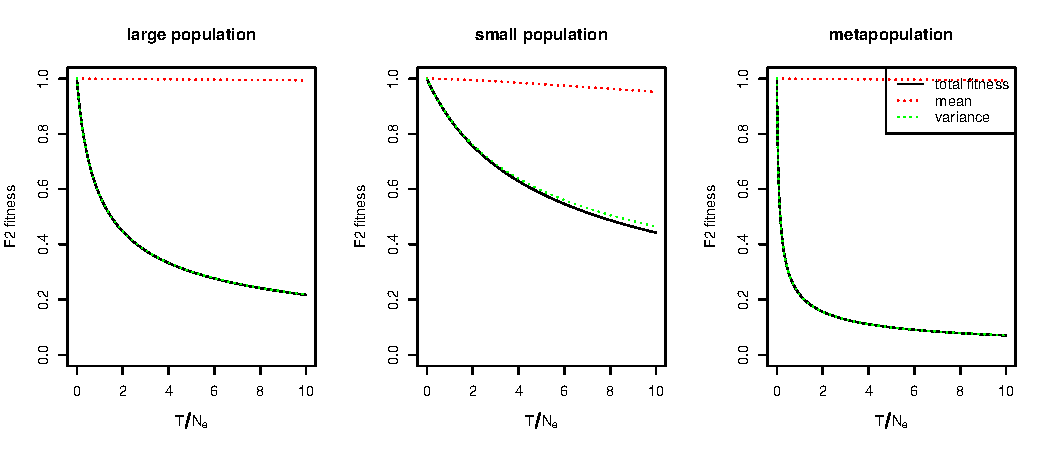
\includegraphics{speciation_rates}
\caption{
Mean drop of $F_1$ and $F_2$ fitness relative to parental species,
with $\omega=1$ and 
\textbf{(A)} $\sigma_N^2 = \sigma_S^2 = \gamma^2$
\textbf{(B)} $\sigma_N^2 = \sigma_S^2 = 0.1 \gamma^2$
\textbf{(C)} $0.1 \sigma_N^2 = \sigma_S^2 = \gamma^2$.
The $F_2$ fitness is from equation \eqref{eqn:fit2},
and the $F_1$ fitness is determined only by the exponential term of that equation.
is small relative to that of increased variance.
\label{fig:speciation_rates}}
\end{center}
\end{figure}


\subsection*{Genetic variation in empirical regulatory systems}

What is known about the key quantity above, the amount of heritable variation in real regulatory networks?
%These are known at best only roughly \citep{felsenstein1988phylogenies},
%so we aim for order-of-magnitude estimates.
The coefficient $A_{ij}$ from the system \eqref{eqn:system} measures how much the rate of net production of $i$ changes
per change in concentration of $j$.
It is generally thought that regulatory sequence change contributes much more to inter- and intraspecific variation
than does coding sequence change affecting molecular structure \citep{schmidt2010fivevertebrate}.
In the context of transcription factor networks this may be affected 
not only by the binding strength of molecule $j$ to the promoter region of gene $i$
but also the effects of other transcription factors (e.g., cooperativity)
and local chromatin accessibility \citep{stefflova2013cooperativity}.
For this reason, 
the mutational target size for variation in $A_{ij}$ may be much larger than the dozens of base pairs
typically implicated in the handful of binding sites for transcription factor $j$ of a typical promoter region,
and single variants may affect many entries of $\allS$ simultaneously.
% (Recall that although these are best modeled through nonlinear terms,
% by linearizing we essentially consider first-order effects.)
% On the other hand, a diverse set of buffering mechanisms are thought to contribute to phenotypic stability
% in the presence of substantial molecular noise \citep{canalization,buffering},
% suggesting that substantial variation in the micro-scale dynamics we consider here
% may be necessary to produce relevant phenotypic effects downstream.

Variation in binding site occupancy may overestimate variation in $A$,
since it does not capture buffering effects (if for instance only one site of many needs to be occupied for transcription to begin),
and variation in expression level measures changes in steady-state concentration (our $\kappa_i$) rather than the \emph{rate} of change.
Nonetheless, these measures likely give us an idea of the scale of variability.
\citet{kasowski2010variation} found differential occupancy in 7.5\%
of binding sites of a transcription factor (p65) between human individuals.
\citet{verlaan2009targeted} showed that cis-regulatory variation
accounts for around 2--6\% of expression variation in human blood-derived primary cells,
while \citet{lappalainen2013transcriptome} found that human population variation 
explained about 3\% of expression variation.
Allele-specific expression is indicative of standing genetic \emph{cis}-regulatory variation;
\citet{wang2017bayesian} found allele-specific expression in 7.2--8.5\% of transcripts of a flycatcher species,
while \citet{tung2015genetic} observed allele-specific expression in 23.4\% of genes studied in a baboon species. 
Taken together, this suggests that variation in the entries of $A$
may be on the order of at least a few percent between individuals of a population --
doubtless varying substantially between species and between genes.

%%%%%%%%%%%%%%%%%%%%%%%%
%%%%%%%%%%%%%%%%%%%%%
\section*{Discussion}

%%% OUTLINE
% - Summarize methods and main result on rate of speciation.
% - Consistent with F1/F2 divergence and Haldane's rule
% - What empirical evidence is there that this is actually happening? 
%   * incompats due to misregulation (Noor, Witkopp...)
%   * numerous species that are visually indistinguishable (skinks, ferns)
%   * maybe also ref phylogenetic lit
% - What other evidence could be collected?  Note could be just phenotype not fitness. (cite Matute)
% - Is linearity an important assumption?
% - We know that divergent selection and genetic conflict can easily lead to speciation; we've shown neutral drift can maybe surprisingly easily do so also; but it remains unclear the relative contributions of these. Note that although drift may be weaker in any one network there are lots of networks. Could motivate this with Orr's statement.  Perhaps tie in spandrels.

Above we synthesize concepts and tools from molecular and evolutionary biology with tools from control theory
to study the evolution of a mechanistic model of the molecular genotype-phenotype map under stabilizing selection.
This model allows us to analytically describe the processes discussed verbally as
phenogenetic drift \citep{weiss2000phenogenetic} and developmental system drift \citep{true2001developmental}.
In this context, the Kalman decomposition \citep{kalman1963mathematical}
gives an analytical description of all phenotypically equivalent gene networks.
It also implies that nearly all systems are nonidentifiable,
and hence the general existence of axes of genetic variation that are not constrained by selection.
The independent movement of separated populations along these axes
can lead to reduction in hybrid viability, and hence speciation,
at a speed that depends on effective population size and amount of genetic variation. 
In this model, at biologically reasonable parameter values,
system drift is a significant -- and possibly rapid -- driver of speciation.
This may at first be surprising because
hybrid inviability appears as a consequence of recombining different, yet functionally equivalent, mechanisms. 

Consistent with empirical observation of hybrid breakdown \citep[e.g.][]{plotner2017chlorosis}, 
we see that the fitnesses of $F_2$ hybrids drop at a much faster rate than those of $F_1$s.
% since $F_1$ and $F_2$ phenotypes diverge linearly and at the square root of time relative to parentals, respectively.
%\plr{refer to Turelli here}
% In this model, this is due to recombination shuffling system architectures, leaving the $F_2$ system homozygous for one parent at one particular locus and homozygous for the other parent at another possibly incompatible locus.
Another natural consequence of the model is Haldane's rule,
that if only one $F_1$ hybrid sex is inviable or sterile it is likely to be the heterogametic sex.
This occurs because if the genes underlying a regulatory network are distributed among both autosomes and the sex chromosome, 
then heterogametic $F_1$s show variation similar to that seen in $F_2$ hybrids.

Is there evidence that this is actually occurring?
System drift and network rewiring has been inferred across the tree of life \citep{wotton2015quantitative, crombach2016gap, dalal2017transcription, johnson2017rewiring, ali2017quantitative},
and there is often significant regulatory variation segregating within populations.
Transcription in hybrids between closely related species with conserved transcriptional patterns can also be divergent 
\citep{haerty2006gene, maheshwari2012cis, coolon2014tempo, michalak2004association, mack2016gene}, and hybrid incompatibilities have been attributed to cryptic molecular divergence underlying conserved body plans \citep{gavin2013embryonic}. 
Furthermore, in cryptic species complexes (e.g., sun skinks \citep{barley2013challenge}),
%strongly reproductively incompatible species
genetically distinct species
may be nearly morphologically indistinguishable.

\paragraph{The origin of species not by means of natural selection?}
% this is neutral, in contrast to other models. although some folks advocate nonadaptive speciation.
% other mechanisms also probly important
% but this one may be strong since happens in all networks at once
Although, as classically formulated, 
the Dobzhansky-Muller model of hybrid incompatibility is agnostic to the relative importance of neutral versus selective genetic substitutions \citep{coyne1998evolutionary},
and plausible mechanisms for the origin of Dobzhansky--Muller incompatibilities by neutral genetic drift have been proposed \citep{lynch2000origin} 
and under stabilizing selection \citep{fierst},
previous authors have argued that neutral processes are likely too slow to be a significant driver of speciation \citep{nei1983models,seehausen2014genomics}.
(Also note that the mechanism underlying hybrid inviability here 
resembles the Dobzhansky-Muller model,
but is more similar to the ``pathway model'' of \citet{lindtke2015genetic}.)
Using simulations, \citet{porter2002speciation} demonstrated the accumulation of hybrid incompatibilities under directional, but not stabilizing selection, and \citet{palmer2009dynamics} observed the appearance of incompatibilities in populations evolving in a constant environment, only if the populations were suboptimally adapted.
This, in light of the few known incompatibilities, has lead some to conclude that hybrid incompatibility is typically a byproduct of positive selection \citep{orr2004speciation, schluter2009evidence} 
or a consequence of genetic conflict \citep{presgraves2010molecular, crespi2013conflictual}.
In contrast, the model we develop here suggests that even under strictly neutral conditions, 
system drift can lead to speciation, at a rate fast enough 
to play a substantial role in species formation across the tree of life. 
Our results show that hybrids, under neutral processes, break down as a function of genetic distance,
and so may, in part, explain broad patterns
such as the relationship between molecular divergence and genetic isolation 
% across diverse taxa and ecologies 
seen by \citet{roux2016shedding}, 
and the clocklike speciation patterns observed by \citet{hedges2015tree}.
% (as diversification is not observed to be accelerated following mass extinctions).

All of these forces -- adaptive shifts, conflict, and network drift --
are plausible drivers of speciation, and may even interact.
For instance, reinforcement due to local adaptation could in some situations provide a selective pressure
that speeds up system drift.
It remains to be seen how the relative strengths of these forces compare.
Furthermore,
while the fitness consequences of incompatibility in any one given network may be small, 
the cumulative impact of system drift across the many different networks an organism relies on may be substantial. 

Of course the basic assumptions of this model will be violated in practice (constant selective pressures, etc.), however, this model can function as a ``neutral null'' description of gene network evolution (a strategy advocated for by \citet{lynch2007frailty, fay2008evaluating, koonin2016splendor}). If this model succeeds in describing actual system evolution, it can be inferred that the mechanism underlying species formation does not require the inclusion of adaptation or changes in selection to explain the emergence of hybrid incompatibility.

\paragraph{Population isolates and genetic load}
Above we have mostly discussed the case of two separated populations of equal size.
In contrast, consider a small subset of a large population that is suddenly isolated.
It will have a large amount of genetic variance, thanks to its history,
but a small population size -- and so can drift quite quickly until it exhausts its genetic variation.
By this point, it could have accumulated substantial incompatibility with the parental population.
Similarly, in a species with substantial isolation by distance, geographically local systems drift
might lead to genetic load due only to recombination, much as in \citep{phillips1996maintenance}.

\paragraph{Nonlinearity and model assumptions}
Of course, real regulatory networks are not linear dynamical systems.
Most notably, physiological limits put upper bounds on expression levels,
implying saturating response curves.
It remains to be seen how well these results carry over into real systems,
but the fact that most nonlinear systems can be locally approximated by a linear one
suggests our qualitative results may hold more generally.
Furthermore, nonidentifiability (which implies the existence of neutral directions)
is often found in practice in moderately complex models of biological systems \citep{gutenkunst2007universally, piazza2008diverse}.

This simple quantitative genetics model we use above
has been shown to produce good predictions in many situations,
even when the substantial number of simplifying assumptions are violated \citep{burger1994distribution,turelli1994genetic}.
The calculations above should be fairly robust even to substantial deviations from normality.
A larger effect on these predictions seems likely due to 
correlations due to molecular constraint, genetic linkage, population structure, historical contingency and so forth.
Although such considerations would not change the qualitative predictions of this model,
their combined effects could substantially change the predicted rate of accumulation of incompatibilities.

Finally, despite our model's precise separation of phenotype and kryptotype, this relationship in nature may be far more complicated as aspects of the kryptotype may be less ``hidden'' than we currently assume. For instance, attributes excluded from the phenotype as modelled here, ignore the potential energy costs associated with excessively large (non-minimal) kryptotypes, as well as the relationship between a specific network architecture and robustness to mutational, transcriptional, or environmental noise.
% Despite the model's simplifications and potentially nontrivial oversights, it may still roughly reflect and shed light upon speciation patterns as they occur in nature.
More precise modeling will require better mechanistic understanding not only of biological systems,
but also the nature of selective pressures
and genetic variation in these systems.

%Maybe compare to \citet{fierst}?
%
%hominids; neanderthal load.

\section*{Acknowledgements}
We would like to thank Sergey Nuzhdin, Stevan Arnold, Erik Lundgren, and Hossein Asgharian for valuable discussion.
%
%\plr{Josh: please fix capitalization in the references.  To do this, anything that needs to be capitalized gets put in curly braces, which tells bibtex to render the capitalization 'as-is'.}

\bibliographystyle{plainnat}
\bibliography{krefs}
%\end{multicols}

\normalsize
\appendix


%%%%%%%%%%%%%%%%%%%%%%%%%%%%%%%
\section{Local expansion of the fitness surface}


%%%%%%%%%%%%%%%%%%%%%%%%%%%%%%%
\subsection{Away from the optimum}
\label{apx:away_from_opt}

Let two points on $\allS$ be $x_1$ and $x_2$, let $\bar x = (x_1+x_2)/2$, and let $z=(x_2 - x_1)/2$.
Then with $\grad D^2$ and $\grad^2 D^2$ the first and second derivatives of $D^2$, respectively,
Taylor expanding about $x_1$ and $x_2$ finds that
\begin{align*}
    D(\bar x)^2 
    &= D(x_1)^2 + \grad D(x_1)^2 \cdot z + \frac{1}{2} z^T \grad^2  D(x_1)^2 z + O(\|z\|^3) \\
    &=  D(x_2)^2 - \grad D(x_2)^2 \cdot z + \frac{1}{2} z^T \grad^2  D(x_2)^2 z + O(\|z\|^3) .
\end{align*}
Now, since $ D(x_1)^2 =  D(x_2)^2 = \grad D(x_1)^2 = \grad D(x_2)^2 = 0$ and
\begin{align*}
    \grad D(x_2)^2 = \grad D(x_1)^2 + 2 z^T \grad^2  D(x_1)^2 + O(\|z\|^2), \quad \text{and} \\
    \grad^2 D(x_2)^2 = \grad^2 D(x_1)^2 + O(\|z\|), 
\end{align*}
adding together the two equations above and dividing by two gets that
\begin{align*}
     D(\bar x)^2
    &= - \frac{3}{2} z^T \grad^2  D(x_1)^2 z + O(\|z\|^3) .
\end{align*}

\subsection{Differentiating the fitness function}
\label{apx:H_calc}

Suppose that $\rho(t) \ge 0$ is a weighting function on $[0,\infty)$
so that fitness is a function of $L^2(\rho)$ distance of the impulse response from optimal.
With $h_0(t) = C_0 e^{tA_0} B_0$ a representative of the optimal set:
\begin{equation}
    \begin{aligned}
        D(A, B, C)^2
        &:= 
        \int_0^\infty \rho(t) \left| h_A(t) - h_0(t) \right|^2 dt \\
        &:= 
        \int_0^\infty \rho(t) \left| C e^{At} B - C_0 e^{A_0 t} B_0 \right|^2 dt \\
        &= 
        \int_0^\infty \rho(t) \tr\left\{
            \left( C e^{At} B - C_0 e^{A_0 t} B_0 \right)^T
            \left( C e^{At} B - C_0 e^{A_0 t} B_0 \right)
        \right\} dt \\
        &= 
        \int_0^\infty \rho(t) \tr\left\{
            \left( C e^{At} B - C_0 e^{A_0 t} B_0 \right)
            \left( C e^{At} B - C_0 e^{A_0 t} B_0 \right)^T
        \right\} dt  ,
        % &= 
        % \int_0^\infty \rho(t)  \tr\left\{
        %         C e^{At} B B^T e^{A^T t} C^T 
        %         - C_0 e^{A_0t} B_0 B^T e^{A^T t} C^T 
        %         \right. \\ &\qquad \qquad \left. {}
        %         - C e^{At} B B_0^T e^{A_0^T t} C_0^T 
        %         + C_0 e^{A_0t} B_0 B_0^T e^{A_0^T t} C_0^T 
        % \right\} dt \\
        % \int_0^\infty \rho(t) \left| C \left( e^{At} - e^{A_0 t} \right) B \right|^2 dt \\
        % &= 
        % \int_0^\infty \rho(t) C \left( e^{At} - e^{A_0 t} \right) B B^T \left( e^{At} - e^{A_0 t} \right)^T C^T dt
    \end{aligned}
\end{equation}
where $\tr X$ denotes the trace of a square matrix $X$.
How does this change as we perturb about $(A_0, B_0, C_0)$?
First we differentiate with respect to $A$, keeping $B=B_0$ and $C=C_0$ fixed.
Since
\begin{equation}
  \begin{aligned}
      \frac{d}{du} e^{(A+uZ)t} \vert_{u=0}
      &=
      \int_0^t e^{As} Z e^{A(t-s)} ds, 
  \end{aligned}
\end{equation}
we have that
\begin{equation}
  \begin{aligned}
      \frac{d}{du} D(A+uZ,B_0,C_0)^2 \vert_{u=0}
      &=
        2 \int_0^\infty \rho(t) \tr\left\{ C_0 \left( \int_0^t e^{As} Z e^{A(t-s)} ds \right) B_0 B_0^T \left( e^{At} - e^{A_0 t} \right)^T C_0^T \right\} dt \\
      &=
        2 \int_0^\infty \rho(t) \tr\left\{ C_0 \left( \int_0^t e^{As} Z e^{A(t-s)} ds \right) B_0 \left( h_A(t) - h_0(t) \right)^T \right\} dt 
  \end{aligned}
\end{equation}
and, by differentiating this and supposing that $A$ is on the optimal set,
i.e., $h_A(t)=h_0(t)$, (so without loss of generality, $A=A_0$):
\begin{equation}
  \begin{aligned}
      \calH^{A,A}(Y,Z) 
      &:= 
      \frac{1}{2} \frac{d}{du} \frac{d}{dv} D(A_0+uY+vZ,B_0,C_0)^2 \vert_{u=v=0} \\
      &=
        \int_0^\infty \rho(t) \tr\left\{ C_0 
        \left( \int_0^t e^{A_0 s} Y e^{A_0 (t-s)} ds \right) 
        B_0 B_0^T 
        \left( \int_0^t e^{A_0 s} Z e^{A_0 (t-s)} ds \right)^T
        C_0^T \right\} dt  .
  \end{aligned}
\end{equation}

The function $\calH$ will define a quadratic form.
To illustrate the use of this, suppose that $B$ and $C$ are fixed.
% Here $\calH$ is the quadratic form underlying the Hamiltonian.
By defining $\Delta_{ij}$ to be the matrix with a 1 in the $(i,j)$th slot
and 0 elsewhere,
the coefficients of the quadratic form is
\begin{equation}
    \begin{aligned}
        H_{ij, k\ell}(A)
        &:=
        \calH(\Delta_{ij}, \Delta_{k\ell}) .
    \end{aligned}
\end{equation}

We could use this to get the quadratic approximation to $D$ near the optimal set.
To do so, it'd be nice to have a way to compute the inner integral above.
Suppose that we diagonalize $A = U \Lambda U^{-1}$.
Then
\begin{equation} \label{eqn:exp_deriv}
  \begin{aligned}
      \int_0^t e^{As} Z e^{A(t-s)} ds 
      &=
      \int_0^t U e^{\Lambda s} U^{-1} Z U e^{\Lambda (t-s)} U^{-1} ds 
  \end{aligned}
\end{equation}
Now, notice that
\begin{equation}
  \begin{aligned}
      \int_0^t e^{s \lambda_i} e^{(t-s) \lambda_j} ds
      &=
      \frac{ e^{t \lambda_i} - e^{t \lambda_j} }{ \lambda_i - \lambda_j } 
          \qquad & \text{if} \quad i \neq j \\
      &=
          t e^{t \lambda_i} 
          \qquad & \text{if} \quad i = j 
  \end{aligned}
\end{equation}
Therefore, 
defining
\begin{equation}
    \begin{aligned}
    X_{ij}(t,Z) 
       &= 
        \left( U^{-1} Z U \right)_{ij}
      \frac{ e^{t \lambda_i} - e^{t \lambda_j} }{ \lambda_i - \lambda_j } 
          \qquad & \text{if} \quad i \neq j \\
      &=
          \left( U^{-1} Z U \right)_{ii}
          t e^{t \lambda_i} 
          \qquad & \text{if} \quad i = j 
    \end{aligned}
\end{equation}
moving the $U$ and $U^{-1}$ outside the integral and integrating we get that
\begin{equation}
  \begin{aligned}
      \int_0^t e^{As} Z e^{A(t-s)} ds 
      &=
      U X(t,Z) U^{-1} .
  \end{aligned}
\end{equation}
This implies that
\begin{equation}
    \begin{aligned}
        D(A_0+\epsilon Z)^2
        &\approx \frac{1}{2} \epsilon^2 
        \int_0^\infty
            \rho(t) \tr\left\{ C U X(t,Z) U^{-1} B B^T (U^{-1})^T X(t,Z)^T U^T C^T \right\}
        dt .
    \end{aligned}
\end{equation}

To compute the $n^2 \times n^2$ matrix $H$,
we see that if $Z=\Delta_{k \ell}$, then
\begin{equation}
  \begin{aligned}
      X_{ij}^{k\ell}(t) 
      &= 
      (U^{-1})_{\cdot k} U_{\ell \cdot}
      \frac{ e^{t \lambda_i} - e^{t \lambda_j} }{ \lambda_i - \lambda_j } 
          \qquad & \text{if} \quad i \neq j \\
      &=
      (U^{-1})_{\cdot k} U_{\ell \cdot}
      t e^{t \lambda_i} 
          \qquad & \text{if} \quad i = j 
  \end{aligned}
\end{equation}
where $U_{k \cdot}$ is the $k$th row of $U$,
and so
\begin{equation}
    \begin{aligned}
        H_{ij, k\ell}(A)
        &=
        \int_0^\infty
            \rho(t) \tr\left\{ C U X^{ij}(t) U^{-1} B B^T (U^{-1})^T X^{k\ell}(t)^T U^T C^T \right\}
        dt .
    \end{aligned}
\end{equation}
This implies that
\begin{equation}
    \begin{aligned}
        D(A_0+\epsilon Z)^2
        &\approx \frac{1}{2} \epsilon^2 \sum_{ijk\ell} H_{ij,k\ell}(A_0) Z_{ij} Z_{k\ell}  .
    \end{aligned}
\end{equation}

By section \ref{ss:quant_gen},
if we set $\Sigma=\sigma^2 I$ and $U=H$,
then a population at $A_0+Z$ experiences a restoring force of strength
$(I + \sigma^2 H^{-1})^{-1} Z$ (treating $Z$ as a vector and $H$ as an operator on these).
If $\sigma^2$ is small compared to $H^{-1}$
then this is approximately $-\sigma^2 H^{-1} Z$.
This suggests that the population mean follows an Ornstein-Uhlenbeck process,
as described (in different terms) in \citet{hansen1996translating}.

More generally, $B$ and $C$ may also change.
To extend this we need the remaining second derivatives of $D^2$.
First, in $B$:
\begin{equation}
    \begin{aligned}
        \mathcal{H}^{B,B}(Y,Z)
        &:= 
        \frac{1}{2} \frac{d}{du} \frac{d}{dv} D(A_0,B_0+uY+vZ,C_0)\vert_{u=v=0} \\
        &=
        \frac{1}{2} \int_0^\infty \rho(t) \tr\left\{ 
        C_0 e^{t A_0}
        \frac{d}{du} \frac{d}{dv} 
        (uY+vZ)
        (uY+vZ)^T
        \vert_{u=v=0} 
        e^{t A_0^T} C_0^T 
        \right\} dt  \\
        &=
        \frac{1}{2} \int_0^\infty \rho(t) \tr\left\{ 
        C_0 e^{t A_0}
        \left( Y Z^T + Z Y^T \right)
        e^{t A_0^T} C_0^T 
        \right\} dt  .
  \end{aligned}
\end{equation}
Next, in $C$:
\begin{equation}
    \begin{aligned}
        \mathcal{H}^{B,B}(Y,Z)
        &:= 
        \frac{1}{2} \frac{d}{du} \frac{d}{dv} D(A_0,B_0,C_0+uY+vZ)\vert_{u=v=0} \\
        &=
        \frac{1}{2} \int_0^\infty \rho(t) \tr\left\{ 
        B_0 e^{t A_0^T}
        \frac{d}{du} \frac{d}{dv} 
        (uY+vZ)^T
        (uY+vZ)
        \vert_{u=v=0} 
        e^{t A_0} B_0
        \right\} dt  \\
        &=
        \frac{1}{2} \int_0^\infty \rho(t) \tr\left\{ 
        B_0 e^{t A_0^T}
        \left( Y Z^T + Z Y^T \right)
        e^{t A_0} B_0
        \right\} dt  .
  \end{aligned}
\end{equation}
Now, the mixed derivatives in $B$ and $C$:
\begin{equation}
    \begin{aligned}
        \mathcal{H}^{B,C}(Y,Z)
        &:= 
        \frac{1}{2} \frac{d}{du} \frac{d}{dv} D(A_0,B_0+uY,C_0+vZ)\vert_{u=v=0} \\
        &=
        \int_0^\infty \rho(t) \tr\left\{ 
        Y e^{t A_0^T} C_0^T Z e^{t A_0} B_0
        \right\} dt  .
  \end{aligned}
\end{equation}
In $A$ and $B$
\begin{equation}
    \begin{aligned}
        \mathcal{H}^{A,B}(Y,Z)
        &:= 
        \frac{1}{2} \frac{d}{du} \frac{d}{dv} D(A_0+uY,B_0+vZ,C_0)\vert_{u=v=0} \\
        &=
        \int_0^\infty \rho(t) \tr\left\{ 
        C_0 \left(\int_0^t e^{s A_0} Y e^{(t-s) A_0} ds \right) B_0
        Z^T e^{t A_0} C_0
        \right\} dt  ,
  \end{aligned}
\end{equation}
and finally in $A$ and $C$:
\begin{equation}
    \begin{aligned}
        \mathcal{H}^{A,C}(Y,Z)
        &:= 
        \frac{1}{2} \frac{d}{du} \frac{d}{dv} D(A_0+uY,B_0,C_0+vZ)\vert_{u=v=0} \\
        &=
        \int_0^\infty \rho(t) \tr\left\{ 
        C_0 \left(\int_0^t e^{s A_0} Y e^{(t-s) A_0} ds \right) B_0
        B_0 e^{t A_0} Z
        \right\} dt  .
  \end{aligned}
\end{equation}

Together, numerical computation of these expressions,
along with estimates of genetic covariance within a population,
allow precise predictions of evolutionary dynamics of a particular system.
The approximation should be good as long as the second-order Taylor approximation holds.


%%%%%%%%%%%%%%%%%%%%%%%%%%%%%%%%%%%%%%%%%%%%%%%%
\section{Genetic drift with a multivariate trait}
\label{ss:quant_gen}

For completeness, we provide a brief exposition of how a population 
evolves due to genetic drift
with a quantitative genetics model,
as in \citet{lande1981models} or \citet{hansen1996translating}.
These do not directly model underlying genetic basis,
but developing a more accurate model is beyond the scope of this paper.

Suppose that the population is distributed in trait space
as a Gaussian with covariance matrix $\Sigma$ and mean $\mu$,
whose density we write as $f(\cdot;\Sigma,\mu)$.
Selection has the effect of multiplying this density by the fitness function and renormalizing,
so that if expected fitness of $x$ is proportional to $\exp(-\|Lx\|^2/2)$,
then the distribution post-selection
has density at $x$ proportional to $f(x;\Sigma,\mu) \exp(-\|Lx\|^2/2)$.
By the computation below (``Completing the square''),
the result is a Gaussian distribution
with covariance matrix $(\Sigma^{-1} + L^T L)^{-1}$ 
and mean $(\Sigma^{-1}+L^T L)^{-1} \Sigma^{-1} \mu$.
% Importantly, if $U$ is not invertible, then by $U^{-1}$ 
% we mean $(U^T U)^{-1} U^T$, Moore-Penrose pseudoinverse of $U$,
% so that $U U^{-1}$ is equal to the projection matrix
% onto the span of the columns of $U$.

After selection, we have reproduction:
suppose this occurs as in the infinitesimal model \citep{barton2016infinitesimal},
so that each offspring of parents with traits $x$ and $y$
is drawn independently from a Gaussian distribution 
with mean $(x+y)/2$ and covariance matrix $R$.
Here, $R$ is the contribution of ``segregation variance'',
i.e., random choices of parental alleles.
If $\widetilde \Sigma = (\Sigma^{-1} + L^T L)^{-1}$ 
is the covariance matrix of the parents post-selection,
then the distribution of offspring will again be Gaussian,
with mean equal to that of the parents
and covariance matrix $\widetilde \Sigma/2 + R$.

In summary, a generation under this model modifies the mean ($\mu$)
and covariance matrix ($\Sigma$) of a population as follows:
\begin{align*}
    \mu &\mapsto \mu' = (\Sigma^{-1}+L^T L)^{-1} \Sigma^{-1} \mu \\
    \Sigma &\mapsto \Sigma' = \frac{1}{2} (\Sigma^{-1} + L^T L)^{-1} + R .
\end{align*}
What measures are stable under this transformation?
The condition $\mu = \mu'$ reduces to $\Sigma L^T L \mu = 0$;
if we assume $R$ and therefore $\Sigma$ are of full rank,
then this happens if and only if $\mu$ is in the null space of $L$,
i.e., if $\mu$ lies in a neutral direction.
The condition $\Sigma' = \Sigma$ can also be solved,
at least numerically.
After rearrangement, it reduces to
$\Sigma L^T L \Sigma + (I/2 - R L^T L) \Sigma = R$.
%% I DON'T THINK WE USE THE FOLLOWING:
% We can find a more explicit description
% if we assume that $x^T L^T L x = \sum_{i=1}^k x_i^2$,
% i.e., that selection only cares about the first $k$ coordinates,
% and then with no interactions between traits.
% If so, the condition $\Sigma' = \Sigma$
% can be written in block form as
% \begin{align*}
%     \begin{bmatrix}
%         \Sigma_{11}^2 + (I/2 - R_{11}) \Sigma_{11}
%         & \Sigma_{11} \Sigma_{12} + (I/2 - R_{11})\Sigma_{12} \\
%         \Sigma_{12}^T \Sigma_{11} + \Sigma_{12}^T/2 - R_{12}^T \Sigma_{11}
%         & \Sigma_{22} - R_{12}^T \Sigma_{12} 
%     \end{bmatrix}
%     &=
%     \begin{bmatrix}
%         R_{11} & R_{12} \\
%         R_{12}^T & R_{22}
%     \end{bmatrix} .
% \end{align*}
% The first equation, $\Sigma_{11}^2 + (I/2 - R_{11}) \Sigma_{11} = R_{11}$,
% can be solved with the quadratic formula: 
% $$\Sigma_{11} = (R_{11} - I/2 + Q)/2$$
% for any $Q$ that commutes with $R_{11}$
% and is a solution to $Q^2 = (R_{11} - I/2)^2 + 4 R_{11}$.
% Since we need $\Sigma$ to be positive definite,
% we take the solution with positive eigenvalues.
% Given $\Sigma_{11}$, the remaining components are
% \begin{align*}
%     \Sigma_{12} 
%     &= 
%     \left( \Sigma_{11} + I/2 - R_{11} \right)^{-1} R_{12} \\
%     \Sigma_{22}
%     &=
%     R_{12}^T \Sigma_{12} + R_{22} .
% \end{align*}
Importantly, the mean $\mu$ does not affect 
either how the covariance matrix moves,
or its stable shape.

Above we have described the \emph{expected} motion of the mean and covariance.
However, random resampling will introduce noise.
Suppose that a population of $N$ individuals
behaves approximately as described above.
By the above,
we may expect that the covariance matrix stays close to a constant value $\Sigma$,
computed from $R$ and $L$ as above,
so that we need only consider motion of the mean, $\mu$.
Since we take a sample of size $N$ to construct the next generation,
the next generation's mean is drawn from a Gaussian distribution with mean $\mu'$
and covariance matrix $\Sigma/N$.
Defining $\Gamma = (I - (I + \Sigma L^T L)^{-1})$,
this can be written as
\begin{align*}
    \mu' - \mu = \Gamma \mu + \epsilon/\sqrt{N} ,
\end{align*}
where $\epsilon$ is a multivariate Gaussian with mean zero and covariance matrix $\Sigma$.
Let $\mu(k)$ denote the mean in the $k^\text{th}$ generation,
and suppose that $\mu$ differs from optimal by something of order $1/\sqrt{N}$:
if $\nu(t) = \sqrt{N} \mu(t\sqrt{N})$ is the rescaled process,
then the previous equation implies that as $N \to \infty$, 
in the limit $\nu$ solves the It\^{o} equation
\begin{align*}
    d \nu(t) = \Gamma \nu(t) dt + \Sigma^{1/2} dW(t) ,
\end{align*}
where now $W(t)$ is a multivariate white noise.
This has an explicit solution as a multivariate Ornstein-Uhlenbeck process:
\begin{align*}
    \nu(t) = e^{-t \Gamma} \nu(0) + \int_0^t e^{-(t-s) \Gamma} \Sigma^{1/2} dW(s).
\end{align*}
% Note that after some algebra, $\Gamma = \Sigma L^T L (I - \Sigma L^T L)^{-1}$.
The asymptotic variance of this process in the direction $z$ is
\begin{align} \label{eqn:limiting_cov}
    \lim_{t \to \infty} \var[\nu(t) \cdot z]
    &=
    \int_0^\infty z^T e^{-s \Gamma} \Sigma e^{-s \Gamma} z ds ,
\end{align}
which is infinite if and only if $\Gamma z = 0$,
which occurs if and only if $Lz=0$.
This implies that at equilibrium, 
population mean trait values lie away from the optimal set
by a Gaussian displacement of order $1/\sqrt{N}$
with a covariance matrix given by equation \eqref{eqn:limiting_cov}.


\paragraph{Completing the square}
First note that if $A$ is symmetric,
\begin{align*}
    (x-y)^T A (x-y)
    &=
    x^T A \left( x - 2y \right) + y^T A y ,
\end{align*}
and so if $B$ is also symmetric and $A+B$ is invertible,
\begin{align*}
    (x-y)^T A (x-y) + x^T B x
    &=
    x^T (A + B) \left( x - 2 (A + B)^{-1} A y \right) + y^T A y \\
    &=
    \left( x - (A + B)^{-1} A y \right)^T
    (A + B)
    \left( x - (A + B)^{-1} A y \right) \\
    &\qquad{}
    + y^T A y - y^T A^T (A+B)^{-1} A y .
\end{align*}
Therefore, 
by substituting $A=\Sigma^{-1}$ and $B=L^T L$,
\begin{align*}
    \frac{ f(x;\Sigma,y) \exp(-x^T L^T L x / 2)}{\int f(z;\Sigma,y) \exp(-z^T L^T L z / 2) dz}
    &=
    f(x; (\Sigma^{-1} + L^T L)^{-1}, (\Sigma^{-1}+L^T L)^{-1} \Sigma^{-1} y) .
\end{align*}

%%%%%%%%%%%%%%%%%%%%%%%%%%%%%%%
\subsection{Gaussian load}
\label{apx:gauss_load}

Suppose that a population has a Gaussian distribution in $d$-dimensional trait space
with mean $\mu$ and covariance matrix $\Sigma$,
and that fitness of an individual at $x$ is $\exp(-\|Lx\|^2/2)$.
Then, completing the square as above with $A=\Sigma^{-1}$, $y=\mu$, and $B=L^T L$,
and defining $Q = (\Sigma^{-1} + L^T L)^{-1}$,
\begin{align*}
    &
    \frac{1}{\sqrt{2 \pi}^n \det(\Sigma)^{1/2}} 
        \int e^{-\frac{1}{2} x^T \Sigma^{-1} x} e^{-\frac{1}{2} x^T L^T L x} dx \\
    &\qquad =
    \frac{1}{\sqrt{2 \pi}^n \det(\Sigma)^{1/2}} 
        \int e^{-\frac{1}{2}(x-Q \Sigma^{-1} \mu)^T Q^{-1} (x-Q \Sigma^{-1} \mu)} dx 
        \\ &\qquad \qquad {}
        \times e^{\mu^T \left( I - \Sigma^{-1} Q \right) \Sigma^{-1} \mu} \\
    &\qquad =
    \sqrt{\frac{\det(Q)}{\det(\Sigma)}}
        \exp\left\{\mu^T \left( I - \Sigma^{-1} Q \right) \Sigma^{-1} \mu\right\} \\
    &\qquad =
    \sqrt{\frac{1}{\det(\Sigma)\det(\Sigma^{-1}+L^TL)}}
        \exp\left\{\mu^T \left( I - (I + L^T L \Sigma)^{-1} \right) \Sigma^{-1} \mu\right\} \\
\end{align*}

Now suppose that $\Sigma = \sigma^2 I$ and $L = I/\gamma$.
Then,
\begin{align*}
    \sqrt{\frac{1}{\det(\Sigma)\det(\Sigma^{-1}+L^TL)}}
    &=
    \sqrt{\frac{1}{\sigma^{2d} (1/\sigma^2 + 1/\gamma^2)^d}} \\
    &=
    \frac{1}{(1+ \left(\sigma/\gamma\right)^2)^{d/2}} .
\end{align*}
Also, 
\begin{align*}
        \left( I - (I + L^T L \Sigma)^{-1} \right) \Sigma^{-1} 
        &=
        \frac{1}{\sigma^2}\left( 1 - (1 + (\sigma/\gamma)^2)^{-1} \right) I \\
        &=
        \frac{1}{\gamma^2}\frac{1}{(1 + (\sigma/\gamma)^2)} I \\
\end{align*}


%%%%%%%%%%%
\section{Evolution of segregation covariance}
\label{apx:seg_cov}

The description above does not describe how \emph{two} diverging populations interact,
since the amount of \emph{segregation variance}, quantified by $R$,
will not stay constant.
To get an idea of how this might change,
suppose that a trait is determined by $L$ unlinked, biallelic loci,
and that the $i^\mathrm{th}$ locus has two alleles with additive effects $\pm x_i$,
so that being homozygous for the $+$ allele contributes $+2x_i$ to the trait.
For simplicity, we will neglect the effects of selection.
If the $+$ allele at locus $i$ is at frequency $p_i$ in a population,
then the mean and genetic variance of the trait in a diploid population with random mating is
\begin{align*}
    m &= 2 \sum_i (2 p_i - 1) x_i \\
    s^2 &= 4 \sum_i p_i (1-p_i) x_i^2 .
\end{align*}


Segregation variance between two parents depends on the loci at which either are heterozygous,
and each locus contributes independently
since alleles are additive.
If the alleles are at Hardy-Weinberg proportions,
then since segregation acts like a fair coin flip, a heterozygous locus contributes $x_i^2/4$ to the variance,
and so the \emph{mean} segregation variance, averaging across parents, is
% two parents, prob 2p(1-p) for prob the locus is heterozygous, variance 0.5(1-0.5)x^2.
\begin{align*}
    R_0(p) = \sum_i p_i (1-p_i) x_i^2 .
\end{align*}

On the other hand,
if the second parent came from a distinct population
with frequencies $q_i$
(an $F_1$ hybrid),
this would be
\begin{align*}
    R_1(p,q) &= \frac{1}{2} \sum_i p_i^2 (1-p_i)^2 x_i^2 
                + \frac{1}{2} \sum_i q_i^2 (1-q_i)^2 x_i^2 \\
                &= (R_0(p) + R_0(q))/2 .
\end{align*}
If we assume that the populations are at equilibrium, $R_0(p) \approx R_0(q)$,
and so $R_1(p,q) \approx R_0(p)$.

Now consider an $F_2$ hybrid, where both parents are $F_1$
and so each heterozygous at locus $i$ with probability $p_i (1-q_i) + (1-p_i) q_i$.
Then
\begin{align*}
    R_2(p,q) &= \frac{1}{2} \sum_i \left(p_i (1-q_i) + (1-p_i) q_i \right) x_i^2  .
\end{align*}
Suppose that the two populations are slightly drifted from each other,
with frequency difference $p_i-q_i = 2\epsilon_i$.
Then,
\begin{align*}
    p (1-q) + p (1-q)
    &=
    (u+\epsilon) (1-u+\epsilon) + (u-\epsilon) (1-u-\epsilon) \\
    &=
    2 u (1-u)
    % + \epsilon (u + (1-u) - u - (1-u))
    + 2 \epsilon^2 .
\end{align*}
If the frequencies have evolved neutrally in unconnected, Wright-Fisher populations 
of effective size $N$ for $t$ generations from a common ancestor with allele frequency $u$,
then $\epsilon$ has mean zero and variance roughly $2 u (1-u) t/N$.
Still assuming the populations are at stationarity,
so that $R_0$ is constant between the two,
and taking the frequencies $p_i$ as a proxy for the ancestral frequencies $u_i$,
this implies that we expect
\begin{align*}
    R_2 
    &\approx 
    R_0 + 2 \sum_i p_i (1-p_i) x_i^2 t/N \\
    &=
    \left( 1 + \frac{2t}{N} \right) R_0 .
\end{align*}
On the other hand, the expected squared difference in trait \emph{means} between two such populations is
\begin{align} \label{eqn:var_dx}
    8 \sum_i p_i (1-p_i) x_i^2 t / N = 8 R_0 t /N .
\end{align}
This implies that under this model,
segregation variance in $F_2$ hybrids between two populations
is roughly increased by a factor of $1/8$ of the difference between their means.



\end{document}



%\section*{Examples}
%\begin{example}[Metabolic network] \label{ex:metabolic}
%Consider an organism that can metabolize two different sugars (present at logarithmic concentrations $u_{1}$ and $u_{2}$), 
%with two enzymes (at log concentrations $\phi_{1}$ and $\phi_{2}$).
%Further suppose that the second sugar is prefered,
%%and that the organism has a regulatory network that can deploy situation specific metabolic strategy.
%and that
%depending on $u_{1}$ and $u_{2}$ the organism will synthesize an appropriate $\phi_{1}$ and $\phi_{2}$. 
%Furthermore, assume this system contains at least two transcription factors, whose log concentrations are $\kappa_{1}$, $\kappa_{2}$, $\dots \kappa_{n}$.
%Minimally such a system may have the architecture,
%%\begin{align*}
%%    \mathcal{S}_{\min} = \left\{ \begin{array}{ll} \dot{\kappa}(t) &= \begin{bmatrix} 0 & -1 \\ 0 & 0 \end{bmatrix} \begin{bmatrix} \kappa_{1} \\ \kappa_{2} \end{bmatrix} (t) + \begin{bmatrix} 1 & 0 \\ 0 & 1 \end{bmatrix} \begin{bmatrix} u_{1} \\ u_{2} \end{bmatrix} (t) \\[11pt]
%%    \phi(t) &= \begin{bmatrix} 1 & 0 \\ 0 & 1 \end{bmatrix} \begin{bmatrix} \kappa_{1} \\ \kappa_{2} \end{bmatrix} (t) \end{array} \right.
%%\end{align*}
%  $\Sys_{\min}(U) = (U \left[ \begin{smallmatrix} 0 & -1 \\ 0 & 0 \end{smallmatrix} \right] U^{-1}, U 
%    %\left[\begin{smallmatrix} 1 & 0 \\ 0 & 1 \end{smallmatrix}\right]
%      ,
%     % \left[\begin{smallmatrix} 1 & 0 \\ 0 & 1 \end{smallmatrix}\right]
%        U^{-1})$. 
%%
%%The impulse response of the system is,
%%$h(t) = \left[\begin{smallmatrix} 1 & - t \\ 0 & 1 \end{smallmatrix}\right]$.
%    We can find alternative equivalent systems by changning coordinates ($U \rightarrow U'$) or, more generally, by applying the Kalman decomposition \ref{apx:kalman}. To illustrate that phenotypic invariance does not require dimensional invariance, we apply the Kalman decomposition to $\Sys_{\min}$ to find 
%    %This may happen if a system is co-opted from another, or may be a consequence of gene duplication and deletion. 
%  $\Sys(\small D_{1-3},V) \! =  \! \left( \! \begin{array}{ll}
%     V \! \left[\begin{smallmatrix} D_{1} & D_{2} \\ 0 & A \end{smallmatrix}\right] \! V^{-1}, V \! \left[\begin{smallmatrix} D_{3} \\ B \end{smallmatrix}\right], \left[\begin{smallmatrix} 0 & C \end{smallmatrix}\right] \! V^{-1} \end{array} \! \right)
%$, both of which are in $\allS$
%%  \begin{align*}
%%    \Sys(X_{1-3},V) = \left( \begin{array}{ll}
%%     V \left[\begin{smallmatrix} X_{1} & X_{2} \\ 0 & A_{\min} \end{smallmatrix}\right] V^{-1}, V \left[\begin{smallmatrix} X_{3} \\ B_{\min} \end{smallmatrix}\right], \left[\begin{smallmatrix} 0 & C_{\min} \end{smallmatrix}\right] V^{-1} \end{array} \right)
%%    \end{align*}
%  ($V$ can be any $4$-dimensional and invertible matrix, $D_{1-3} \in \R^{2 \times 2}$, and $(A,B,C) \in \Sys_{\min}$).
%%So for example, some system can be wired as follows, and still be input-output equivalent to the minimal metabolic system $\mathcal{S}_{\min}$:
%% \begin{align*}
%%   A' &= \begin{bmatrix}
%%     1.6923  &  1.5385 &  -2.6154 &  -2 \\
%%     0.8462  &  0.7692 &  -1.3077 &  -1 \\
%%     1.2692  &  1.1538 &  -1.9615 &  -1.5 \\
%%     0.4231  &  0.3846 &  -0.6538 &  -0.5
%%   \end{bmatrix} \\
%%   B' &= \begin{bmatrix} 4 & 4 \\ 2 & 2 \\ 3 & 3 \\ 1 & 3 \end{bmatrix} \\
%%     C' &= \begin{bmatrix}  0.2692  &  0.1538  &  0.0385 &  -0.5 \\
%%     -0.4231 &  -0.3846 &   0.6538  &  0.5 \end{bmatrix}
%% \end{align*}
%%
%%Despite the present example consisting of a minimal $2 \times 2$ and a non-minimal $4 \times 4$ system, 
%%any $m$-dimensional system can be constructed using this method 
%%-- applying a change of coordinates to the Kalman decomposition 
%%-- to construct a mechanistically different system with identical phenotypic dynamics. 
%%
%%When applying the Kalman decomposition to real biological networks, one may have to restrict the free parameters, as physiology and biochemistry might not allow all mathematically possible coefficients. We note that as there are so many degrees of freedom, it may be difficult to infer system function solely from structure. 
%\end{example}


